\documentclass[11pt]{article}

\usepackage[T1]{fontenc}
\usepackage{lmodern}
\usepackage{microtype}
\usepackage[margin=1in]{geometry}
\usepackage{amsmath,amssymb,amsthm,mathtools}
\usepackage{aliascnt}
\usepackage{booktabs,tabularx,array}
\usepackage{graphicx}
\usepackage{enumitem}
\usepackage[authoryear]{natbib}
\usepackage{xcolor}
% Changes relative to main(4).tex are blue. For a clean copy, replace this
% definition with: \newcommand{\pRevision}[1]{#1}
\newcommand{\pRevision}[1]{{\color{blue}#1}}
\usepackage[colorlinks=true,linkcolor=blue!55!black,citecolor=blue!55!black,urlcolor=blue!55!black]{hyperref}
\usepackage{doi}
\usepackage{hyperxmp}
\usepackage[nameinlink,noabbrev,capitalize]{cleveref}

\hypersetup{
	pdftitle={A global spectral gap for Metropolis-adjusted Langevin algorithm with a uniformly randomized step size},
	pdfauthor={Qian Qin and Guanyang Wang},
	pdfsubject={Spectral-gap bounds for randomized-step MALA},
	pdfkeywords={Markov chain Monte Carlo, MALA, spectral gap, conductance, randomized step size},
	pdfdisplaydoctitle=true,
	pdflang={en-US},
	bookmarksopen=true,
	bookmarksnumbered=true
}

\allowdisplaybreaks
\setlength{\parindent}{1.5em}
\setlength{\parskip}{0pt}
\setlength{\emergencystretch}{2em}

\newtheorem{theorem}{Theorem}[section]
\newaliascnt{lemma}{theorem}
\newtheorem{lemma}[lemma]{Lemma}
\aliascntresetthe{lemma}
\newaliascnt{proposition}{theorem}
\newtheorem{proposition}[proposition]{Proposition}
\aliascntresetthe{proposition}
\newaliascnt{corollary}{theorem}
\newtheorem{corollary}[corollary]{Corollary}
\aliascntresetthe{corollary}
\newaliascnt{remark}{theorem}
\newtheorem{remark}[remark]{Remark}
\aliascntresetthe{remark}
\crefname{theorem}{Theorem}{Theorems}
\crefname{lemma}{Lemma}{Lemmas}
\crefname{proposition}{Proposition}{Propositions}
\crefname{corollary}{Corollary}{Corollaries}
\crefname{remark}{Remark}{Remarks}


\newcommand{\R}{\mathbb R}
\newcommand{\E}{\mathbb E}
\newcommand{\Var}{\operatorname{Var}}
\newcommand{\Gap}{\operatorname{Gap}_{\mathrm{R}}}
\newcommand{\TV}{\operatorname{TV}}
\newcommand{\cE}{\mathcal E}
\newcommand{\cK}{\mathcal K}
\newcommand{\ip}[2]{\left\langle #1,#2\right\rangle}
\newcommand{\norm}[1]{\left\lVert #1\right\rVert}
\newcommand{\abs}[1]{\left\lvert #1\right\rvert}
\newcommand{\1}{\mathbf 1}
\newcommand{\df}{\mathrm{d}}

\title{A global spectral gap for Metropolis-adjusted Langevin algorithm with a uniformly randomized step size}
\author{Qian Qin \\ School of Statistics \\ University of Minnesota}
\date{}
\hypersetup{pdfauthor={Qian Qin}}
\ifdefined\pdfinfo
\pdfinfo{/Author (Qian Qin)}
\fi

\begin{document}
	\maketitle
	
	\begin{abstract}
		Let \(\pi(\df x)\propto e^{-U(x)}\,\df x\) on \(\R^d\), where
		\(U\) is continuously differentiable and \(m\)-strongly convex with a globally
		\(L\)-Lipschitz gradient, \(0<m\leq L<\infty\), and \(\kappa=L/m\).
		It is known that, under warm-start assumptions, fixed-step Metropolis-adjusted Langevin algorithm (MALA) with properly tuned step size has mixing time of order $\kappa \sqrt{d}$ up to logarithmic factors.
		By contrast, when the condition number is bounded away from one, no single fixed step size yields a matching spectral-gap lower bound of order $(\kappa \sqrt{d})^{-1}$ uniformly over this target class.
		We show that MALA with a uniformly randomized step size admits a spectral-gap lower bound of this size.
		At each iteration, the randomized-step MALA considered here draws \(h\) uniformly from
		\((0,H)\) and performs one ordinary MALA transition with step size \(h\).
		We show that, when \(H\) is of order \((L\sqrt{d})^{-1}\), the right spectral gap of randomized-step MALA admits a lower bound of order
		\[
		\frac{1}{\kappa\sqrt{d}\,[1+\log(d+1)+\log\kappa]}.
		\]
		A key ingredient in the proof is a
		Cheeger-type inequality for aggregating estimates of the one-step flow
		of MALA out of measurable sets at various step-size scales.  It allows
		the scale used to control the flow to depend on the set and avoids the
		additional loss that would result from first estimating the conductance and then
		applying the standard Cheeger inequality.
		This work was developed with substantial assistance from ChatGPT, which suggested the uniformly randomized-step approach, developed the principal proof arguments, and generated the simulation and Lean 4 code. The human author checked and verified the mathematical content and takes full responsibility for the results.
	\end{abstract}
	
	\section{Introduction}
	
	For a target probability distribution~$\pi$ on $\R^d$ with density proportional to \(e^{-U}\), the
	Metropolis-adjusted Langevin algorithm (MALA) proposes
	\[
	Y=x-h\nabla U(x)+\sqrt{2h}\,Z,
	\; \text{ where } Z\sim N_d(0,I_d),
	\]
	and applies the Metropolis--Hastings correction.  
	MALA is one of the most fundamental Markov chain Monte Carlo (MCMC)
	algorithms and has been studied extensively.
	Its classical geometric
	properties and high-dimensional scaling were developed by
	\citet{RobertsTweedie1996,RobertsRosenthal1998}; it is also closely related to Hamiltonian Monte Carlo
	\citep{Neal2011,WuSchmidlerChen2022,ChenGatmiry2023}.
	
	
	For an \(m\)-strongly convex and \(L\)-smooth potential $U(\cdot)$, \citet{WuSchmidlerChen2022}, strengthening results in \cite{ChewiEtAl2021}, show that the mixing time of (lazy) MALA from a warm start has the
	minimax \(\kappa\sqrt{d}\) dependence, up to logarithmic factors, where $\kappa = L/m$ is the condition number.
	This rate is achieved with a MALA step size~$h$ of order \((L\sqrt{d})^{-1}\) up to logarithmic factors.
	The proofs in \cite{ChewiEtAl2021} and \cite{WuSchmidlerChen2022} control acceptance on a high-probability region and then use an $s$-conductance argument \citep{LovaszSimonovits1993}.  
	They therefore do not lower-bound the ordinary conductance over sets of every positive stationary mass, and their arguments do not yield a matching global Poincar\'e bound of the form 
	\begin{equation} \label{eq:gap-ideal}
		\Gap(P_h)\gtrsim \frac{1}{\kappa \sqrt{d}},
	\end{equation}
	where $P_h$ is the Markov kernel of MALA with step size~$h$,  $\Gap(\cdot)$ denotes the right spectral gap, and $\gtrsim$ suppresses
	universal constants and the logarithmic factors.
	(Recall that, for a lazy reversible Markov chain, the mixing time is roughly inversely proportional to the right spectral gap, so a gap of order $(\kappa \sqrt{d})^{-1}$ implies mixing time of order $\kappa \sqrt{d}$.)
	Under only strong convexity and gradient Lipschitzness, a fixed-step global Poincaré bound at the $d^{-1/2}$
	scale is impossible uniformly over the target class. Indeed, following arguments from \cite{ChewiEtAl2021,WuSchmidlerChen2022}, we show that a bound of the form \eqref{eq:gap-ideal} cannot hold uniformly over all $m$-strongly convex and $L$-smooth potentials if $\kappa - 1$ is greater than a positive constant.
	In fact, in Proposition \ref{prop:minimax-fixed-step-ceiling}, it is shown that, when $\kappa \geq \kappa_0 > 1$ for some constant $\kappa_0$, for any $h > 0$, there exists an $m$-strongly convex and $L$-smooth potential~$U$ such that $\Gap(P_h)$ is upper bounded by a $\kappa_0$-dependent multiple of the maximum of $\log(\kappa d)/(\kappa d)$ and $e^{-cd}$, where $c > 0$ is universal.
	
	A global spectral-gap bound is useful for more than deriving a mixing-time estimate. 
	Let \(P\) be a lazy (or positive semi-definite), \(\pi\)-reversible Markov kernel. 
	If $\mu$ is an initial distribution with $\df\mu/\df\pi\in L^2(\pi)$, then
	\begin{equation} \label{eq:TVbound}
		\norm{\mu P^n-\pi}_{\mathrm{TV}}
		\leq
		\frac12\norm{\frac{\df\mu}{\df\pi}-1}_{L^2(\pi)}
		[1-\Gap(P)]^n.
	\end{equation}
	Thus a spectral gap certifies convergence all the way to stationarity, rather than only for a prescribed accuracy \citep{KontoyiannisMeyn2012,RobertsRosenthal1997Hybrid,Rudolf2012}. 
	More importantly for Monte Carlo, for a stationary reversible chain and a centered function in $L^2(\pi)$, a positive right spectral gap implies a central limit theorem for Markov-chain averages and controls their asymptotic variance \citep{KipnisVaradhan1986}. 
	Related spectral arguments also yield finite-sample variance, mean-square error, and concentration bounds for Markov-chain averages \citep{Rudolf2012,Paulin2015}. 
	By contrast, a favorable warm-start mixing bound can coexist with very high autocorrelation for certain $L^2(\pi)$ test functions.
	
	Quantitative global spectral-gap results for MALA are considerably sparser than mixing-time bounds. 
	The classical analysis of \citet{RobertsTweedie1996} gives qualitative criteria for geometric ergodicity, rather than dimension-explicit lower bounds on the gap, while \citet{BouRabeeHairer2013} show that, for drifts that are not globally Lipschitz, MALA may fail to have a spectral gap even when the underlying Langevin diffusion does. 
	\citet{WuSchmidlerChen2022} use spectral-gap upper bounds of order $mh$ for
	specially constructed targets to establish their minimax mixing-time lower
	bound, but the existing fixed-step analyses do not provide a matching global
	spectral-gap lower bound when~$h$ is of order $(L\sqrt{d})^{-1}$.
	More recently, \citet{LiuTong2026} establish $\Gap(P_h)\gtrsim(\kappa^2d)^{-1}$ when
	$h$ is of order $(\kappa Ld)^{-1}$.
	This spectral-gap bound gives a
	mixing-time bound of order $\kappa^2d$, which is significantly worse than the
	$\kappa\sqrt{d}$ dependence achieved with a step size of order
	$(L\sqrt{d})^{-1}$.
	
	
	We study the randomized kernel
	\[
	\overline P_H=\frac1H\int_0^H P_h\,\df h.
	\] 
	Operationally, the algorithm samples
	\(h\sim\operatorname{Unif}(0,H)\) and then performs one ordinary MALA
	step.  It uses one proposal and has essentially the same computational cost
	as fixed-step MALA.  
	By linearity of detailed balance, it is exactly \(\pi\)-reversible.
	In \cref{thm:main}, we show that if $U$ is continuously differentiable, $m$-strongly convex, and has an $L$-Lipschitz gradient, and $H$ is of order
	$(L\sqrt{d})^{-1}$, then $\Gap(\overline P_H)$ has a lower bound of order
	$(\kappa\sqrt{d})^{-1}$, up to logarithmic factors, matching the minimax
	mixing-time bound for fixed-step MALA.
	
	
	
	
	Randomization of Metropolis tuning parameters has been advocated as a
	way to improve robustness.  In the setting most directly relevant here,
	\citet{GrazziLivingstoneRiouDurand2026} study the
	randomized kernel $\int P_h\,\nu(\df h)$, where~$\nu$ is a distribution on $(0,\infty)$.  
	They show that randomized
	kernels inherit spectral gaps and weak Poincar\'e inequalities from suitable
	fixed-step components and that randomization can turn
	severe sensitivity to step-size misspecification into a much milder deterioration of the spectral gap.  
	The intuition is that a randomized method may sacrifice some
	peak asymptotic efficiency in exchange for performing reasonably over a
	much wider range of scales.  
	Related benefits of randomization are known
	for Hamiltonian methods \citep{BouRabeeSanzSerna2017,ApersGriblingSzilagyi2024}.  
	
	As shown in \cite{GrazziLivingstoneRiouDurand2026}, the randomized kernel satisfies the inheritance bound $\Gap(\overline P_H) \geq H^{-1} \int_0^H \Gap(P_h) \, \df h$.
	This inequality alone, however, does not yield the $(\kappa\sqrt{d})^{-1}$
	rate sought here, because no available fixed-step result establishes
	$\Gap(P_h)\gtrsim(\kappa\sqrt{d})^{-1}$, regardless of~$h$.
	To be more specific, existing conductance lower bounds, which are translated into spectral-gap lower bounds via Cheeger’s inequality \citep{LawlerSokal1988}, are considerably smaller than desired at every scale.
	Recall that Cheeger's inequality asserts that $\Gap(P_h)$ is lower bounded by $\phi(P_h)^2/2$, where $\phi(P_h)$ is the global conductance:
	\[
	\phi(P_h) := \inf_{S: \, 0 < \pi(S) \leq 1/2} \frac{\mathcal{J}_{P_h}(S, S^c)}{\pi(S)}, \quad \mathcal{J}_{P_h}(S, S^c)=  \int_S P_h(x, S^c) \, \pi(\df x).
	\]
	To apply Cheeger's inequality, we want a lower bound on $\phi(P_h)$ that is of order $(\kappa \sqrt{d})^{-1/2}$ for a sufficiently large set of $h \in [0,H]$.
	More precisely, \citet{LiuTong2026} obtain a lower bound on $\phi(P_h)$ of
	order $(\kappa^2d)^{-1/2}$ for $h\lesssim(\kappa Ld)^{-1}$.  For $h$ of
	order $(L\sqrt{d})^{-1}$, \citet{WuSchmidlerChen2022} obtain a lower bound of
	order $(\kappa\sqrt{d})^{-1/2}$ on $\mathcal{J}_{P_h}(S,S^c)/\pi(S)$ when $\pi(S)$
	exceeds a certain threshold; below that threshold, however, the ratio can
	scale very poorly with~$d$.
	
	Our argument exploits information that the preceding inheritance bound discards: the step-size range used to control the flow out of a set may depend on the stationary mass of that set.
	For each measurable $S \subset \R^d$, we select a range of step sizes tailored to $\pi(S)$, using progressively smaller steps as $\pi(S)$ decreases.
	When $\pi(S)$ is not too small, comparatively larger steps can be used: the Metropolis acceptance rate is lower bounded by a positive constant over~$S$, outside an exceptional set with small stationary mass \citep{ChewiEtAl2021,WuSchmidlerChen2022}.
	Writing $\cK_t=(2/t)\int_{t/2}^tP_h\,\df h$ for the kernel averaged over the upper dyadic half of $(0,t)$, one can then lower-bound the one-step flow $\mathcal{J}_{\cK_t}(S,S^c)$ by a suitable multiple of $\pi(S)$.
	For smaller sets, the exceptional region in the preceding argument can no longer be ignored, and we instead use a smaller, globally safe step size which leads to a constant uniform lower bound on the acceptance rate over the whole space.
	Gaussian isoperimetry then supplies the corresponding lower bound on the flow out of~$S$.
	
	Finally, we combine the flow estimates obtained at the different scales
	using a Cheeger-type aggregation lemma (\cref{lem:fractional}) for mixtures of reversible Markov
	kernels. 
	The lemma lets
	us use relatively large steps for sets of moderate stationary mass and
	smaller steps for rarer sets, without losing an additional factor that would result from first estimating the conductance and then applying the standard Cheeger inequality.
	The closest
	analytic predecessor is the general Cheeger inequality of
	\citet{ChenWang2000}, which can be used to derive \cref{lem:fractional}.
	We give a direct proof and a more transparent formulation (\cref{thm:aggregation}) suitable for the present setting.
	
	
	An accompanying Lean~4 development provides proof scripts for the main
	theorem and other principal theorem-level conclusions, including
	\cref{thm:main,prop:minimax-fixed-step-ceiling,lem:fractional,thm:aggregation}.
	The scope of these scripts and the verification status of the revised
	first-order interface are described in \cref{sec:lean-verification}.
	
	%\subsection*{Contributions}
	%
	%The proof has four main parts.
	%
	%\begin{enumerate}[label=\textnormal{(\roman*)},leftmargin=2.4em]
	%\item We prove a global Poincar\'e lower bound for uniform-random MALA that,
	%in the regime
	%\(1+\log(d+1)+\log\kappa\lesssim d\), is within one logarithmic factor
	%of the warm-start minimax dimension dependence.  The theorem holds for
	%every endpoint \(H>0\), and explicitly describes both under-tuning and
	%over-tuning.
	%
	%\item We replace a single high-probability acceptance region by a
	%moment-indexed local-overlap statement.  For every \(p\geq1\), a step of
	%order \(\{L\sqrt{p(d+p)}\}^{-1}\) has good local overlap outside a set
	%whose stationary mass decays exponentially in \(p\).  The proof starts
	%from an \(L^p(\pi)\) bound for the pointwise, momentum-averaged rejection
	%probability.  This is the conditional quantity needed by the conductance
	%argument.
	%
	%\item We assign sets to a geometric ladder of step-size intervals according
	%to \(\log(1/\pi(S))\).  Moderate sets use larger steps and smaller sets
	%use larger moment orders and smaller steps.  A globally safe interval of
	%order \((Ld)^{-1}\) controls the final tail of set sizes.
	%
	%\item We use a harmonic component-aggregation lemma.  Conductances of the
	%assigned components are combined before the final Cauchy--Schwarz step, so
	%the probabilities with which useful intervals are selected enter linearly
	%rather than being squared by a direct application of Cheeger's inequality
	%\citep{LawlerSokal1988}.
	%\end{enumerate}
	
	%The constants are universal.  All dependence on \(d,m,L,\kappa,H\), and the
	%moment order is explicit.
	
	\subsection*{Relation to existing work}
	
	Controlling the rejection rate is central to the analysis of MALA.
	There are several approaches to controlling MALA rejection at the
	\(d^{-1/2}\) step-size scale.  \citet{ChewiEtAl2021} use a projection
	characterization of Metropolis adjustment and compare the Euler proposal
	with exact Langevin diffusion.  \citet{WuSchmidlerChen2022} instead compare
	one leapfrog step with continuous Hamiltonian dynamics.
	%\citet{ChenGatmiry2023} develop a finite-dimensional
	%integration-by-parts calculation.  No acceptance estimate from that paper is
	%used here.  
	Earlier pathwise comparisons between
	Metropolized integrators and their limiting diffusions include
	\citet{BouRabeeVandenEijnden2010,BouRabeeHairer2013}.
	
	
	Our appendix follows the diffusion-comparison philosophy.
	The stationary increment estimate follows from the
	Lyons--Zheng forward--backward decomposition
	\citep[Section~1, especially equation~(1.7)]{LyonsZheng1988};
	see also \citet[Theorem~5.7.1]{FukushimaOshimaTakeda2011}.
	We give an elementary proof for Langevin diffusion by writing
	the stochastic differential equation along the forward and reversed
	paths and subtracting the resulting expressions to cancel the drift.
	A
	Girsanov change of path law then compares the exact diffusion with the drift
	frozen at its initial state.  Endpoint conditioning and the
	Metropolis--Hastings meet identity
	\citep{Tierney1998,BilleraDiaconis2001} convert the path estimate into an
	\(L^p(\pi)\) rejection bound.  
	%Quantitative martingale inequalities
	%introduce an additional factor \(\sqrt{p}\); this is the source of the final
	%logarithmic loss.
	
	The close-coupling and isoperimetric part of the argument is standard in
	modern Metropolis analyses
	\citep{DwivediEtAl2019,WuSchmidlerChen2022,AndrieuLeePowerWang2024,LiuTong2026}.
	The use of a scale indexed by set size is related in spirit to average
	conductance, evolving sets, blocking conductance, and spectral profiles
	\citep{LovaszKannan1999,MorrisPeres2005,GoelMontenegroTetali2006,KannanLovaszMontenegro2006}.
	
	The closest analytic predecessor of our aggregation lemma is
	\citet{ChenWang2000}.  They prove a general version of Cheeger's inequality
	that applies in settings considerably broader than the Markov-kernel
	setting considered here and extends the earlier results of
	\citet{LawlerSokal1988}.  Their result can be used to derive our aggregation
	lemma, although the proof we give is direct and self-contained.  The part
	specific to our argument is the way the lemma is combined with the
	set-dependent choice of scale: different sets may require different
	step-size ranges.  We use this idea to combine flow estimates over a
	geometric sequence of step-size ranges for randomized-step MALA.
	
	\subsection*{Generative AI disclosure}
	
	This project began when the author asked ChatGPT 5.6 Sol (OpenAI) whether MALA admits a useful global spectral-gap bound at the $d^{-1/2}$ step-size scale. ChatGPT suggested studying a uniformly randomized-step version of MALA—an algorithmic variant that had previously appeared in the literature—and developed the principal proof strategy and initial versions of the major mathematical arguments in this article. It also assisted in drafting and revising the manuscript and generated all code used for the numerical experiments and the Lean 4 formal verification. The human author checked the relevant literature, scrutinized and revised the AI-generated arguments, verified the mathematical claims and computations, inspected the simulation methodology and results, and confirmed that the Lean development was kernel-checked without proof placeholders or problem-specific axioms. The human author takes full responsibility for the content and correctness of the article.
	
	
	\section{Setup and Main Result}
	
	Assume throughout, except where explicitly stated otherwise, that \(d\) is a
	positive integer and that \(U:\R^d\to\R\) is continuously differentiable,
	\(m\)-strongly convex, and has a globally \(L\)-Lipschitz gradient, where
	\(0<m\leq L<\infty\). Explicitly, for every \(x,y\in\R^d\),
	\begin{equation}\label{eq:first-order-assumptions}
		\begin{aligned}
			&U(y)\geq U(x)+\ip{\nabla U(x)}{y-x}+\frac m2\norm{y-x}^2,\\
			&\norm{\nabla U(y)-\nabla U(x)}\leq L\norm{y-x}.
		\end{aligned}
	\end{equation}
	%	We also use the standard consequence
	%	\begin{equation}\label{eq:first-order-upper-taylor}
		%		U(y)\leq U(x)+\ip{\nabla U(x)}{y-x}+\frac L2\norm{y-x}^2.
		%	\end{equation}
	%	Indeed, integrate
	%	\(\ip{\nabla U(x+s(y-x))-\nabla U(x)}{y-x}\) over \(s\in[0,1]\)
	%	and apply the gradient-Lipschitz bound; see also
	%	\citet[Theorem~2.1.5]{Nesterov2004}.
	%	No second derivative of \(U\) is assumed. The Hessian inequalities
	%	\(mI_d\preceq\nabla^2U\preceq LI_d\) are a sufficient special case
	%	when \(U\in C^2\). 
	Strong convexity implies that \(e^{-U}\) is integrable.
	Let \(\kappa:=L/m\geq1\), and define the target distribution
	\[
	\pi(\df x)=\frac{e^{-U(x)}}{\int_{\R^d}e^{-U(u)}\,\df u}\,\df x.
	\]
	For \(h>0\), let \(Q_h(x,\cdot)\) be the Gaussian law
	\[
	N_d \bigl(x-h\nabla U(x),2hI_d\bigr).
	\]
	The fixed-step MALA kernel is
	\[
	P_h(x,\df y)=\alpha_h(x,y) \, Q_h(x,\df y)
	+\left[1-\int\alpha_h(x,z) \, Q_h(x,\df z)\right]\delta_x(\df y),
	\]
	where
	\[
	\alpha_h(x,y)
	=1\wedge
	\frac{e^{-U(y)} \, q_h(y,x)}{e^{-U(x)} \, q_h(x,y)}
	\]
	and \(q_h\) is the density of \(Q_h\).  The usual
	Metropolis--Hastings argument makes \(P_h\) \(\pi\)-reversible
	\citep{Tierney1998}; consequently, so is the randomized-step MALA kernel
	$$\overline P_H(x,\df y)=\frac{1}{H}\int_0^H P_h(x, \df y)\,\df h.$$
	
	For probability measures \(\mu,\nu\) on a measurable space $(\Omega,\mathcal{F})$, write
	\[
	\TV(\mu,\nu)=\sup_{A \in \mathcal{F}}\abs{\mu(A)-\nu(A)}.
	\]
	For a probability measure $\varpi$, let $L^2(\varpi)$ be the space of
	measurable functions $f:\Omega\to\R$ such that
	$\int f^2\,\df\varpi<\infty$.  For a $\varpi$-reversible kernel $P$ and
	$f\in L^2(\varpi)$, define the Dirichlet form
	\[
	\cE_P(f,f)
	=\frac12\int[f(x)-f(y)]^2\,\varpi(\df x)P(x,\df y).\]
	The right, or Poincar\'e, spectral gap is defined as  
	\[
	\Gap(P)=\inf_{\substack{f\in L^2(\varpi)\\ \Var_\varpi(f)>0}}
	\frac{\cE_P(f,f)}{\Var_\varpi(f)}.
	\]
	This quantity lies in $[0,2]$, and controls the convergence properties of the Markov chain associated with~$P$ if~$P$ is lazy or positive semidefinite.
	%See \citet{LawlerSokal1988} for the relation between this
	%variational quantity and conductance.
	
	%The next elementary lemma will be used repeatedly. 
	%
	%\begin{lemma} \label{lem:mixture-Dirichlet}
	%\label{lem:mixture-dirichlet}
	%Let \(H>0\), and let \(I_1,\ldots,I_N\) be pairwise disjoint Borel subsets
	%of \((0,H)\) with positive Lebesgue measure.  Define
	%\[
	% K_{I_j}=\frac1{|I_j|}\int_{I_j}P_h\,\df h.
	%\]
	%Then every \(K_{I_j}\) is \(\pi\)-reversible and, for every
	%\(f\in L^2(\pi)\),
	%\begin{equation}\label{eq:mixture-dirichlet-identity}
	% \cE_{\overline P_H}(f,f)
	% =\frac1H\int_0^H\cE_{P_h}(f,f)\,\df h
	% \geq
	% \sum_{j=1}^N\frac{|I_j|}{H}\cE_{K_{I_j}}(f,f).
	%\end{equation}
	%\end{lemma}
	
	%\begin{proof}
	%For each \(h>0\), detailed balance gives the equality of measures
	%\[
	% \pi(\df x)P_h(x,\df y)=\pi(\df y)P_h(y,\df x).
	%\]
	%Integrating this identity over \(I_j\) proves reversibility of \(K_{I_j}\).
	%For the Dirichlet form, the integrand
	%\((f(x)-f(y))^2\) is nonnegative.  Tonelli's theorem therefore permits the
	%order of integration in \(h,x,y\) to be exchanged, even when the energy is
	%infinite, and gives
	%\[
	%\begin{aligned}
	% \cE_{\overline P_H}(f,f)
	% &=\frac1{2H}\int_0^H\int
	%   (f(x)-f(y))^2\,\pi(\df x)P_h(x,\df y)\,\df h\\
	% &=\frac1H\int_0^H\cE_{P_h}(f,f)\,\df h.
	%\end{aligned}
	%\]
	%Restricting the last integral to the disjoint union
	%\(I_1\cup\cdots\cup I_N\), and applying Tonelli once more, yields
	%\[
	% \frac1H\sum_{j=1}^N\int_{I_j}\cE_{P_h}(f,f)\,\df h
	% =\sum_{j=1}^N\frac{|I_j|}{H}\cE_{K_{I_j}}(f,f),
	%\]
	%which proves \eqref{eq:mixture-dirichlet-identity}.
	%\end{proof}
	
	The main result of this paper is stated below.
	Its proof is given in \cref{sec:ingredients,sec:main-proof}.
	
	\begin{theorem} \label{thm:main}
		There are universal constants $A_0 \in [1,\infty)$, $b_0 \in (0,1/2]$, and
		\(c_0 > 0\) such that the following holds.  Define
		\begin{equation*}
			p_\star=A_0[1+\log(d+1)+\log\kappa].
		\end{equation*}
		Then, for every \(H>0\),
		\begin{equation}\label{eq:master-gap}
			\Gap(\overline P_H)
			\geq
			c_0\frac{m}{H}
			\min\left\{
			H,
			\frac{b_0}{L}
			\max\left\{
			\frac{1}{\sqrt{p_\star(d+p_\star)}},
			\frac1d
			\right\}
			\right\}^{2}.
		\end{equation}
		For the lazy kernel \((I+\overline P_H)/2\), the right-hand side is
		divided by two.
	\end{theorem}
	
	\begin{corollary}\label{cor:sqrt-d-endpoint}
		Under the assumptions and notations of Theorem~\ref{thm:main}, let
		$H=c/(L\sqrt{d})$ for some $c>0$.
		Then
		\[
		\Gap(\overline P_H) \geq \frac{c_0}{\kappa\sqrt{d}}
		\min \left\{ c, \frac{b_0^2}{c}
		\max \left\{ \frac{d}{p_\star(d+p_\star)}, \frac{1}{d} \right\} \right\}.
		\]
		In particular, since $\min\{p_\star(d+p_\star)/d,d\}\leq2p_\star$,
		\[
		\Gap(\overline P_H) \geq \frac{c_0}{\kappa\sqrt{d}}
		\min\left\{ c, \frac{b_0^2}{2cp_\star} \right\}.
		\]
	\end{corollary}
	
	The spectral gap lower bound of order $(\kappa \sqrt{d})^{-1}$, up to logarithmic factors, for randomized-step MALA is in sharp contrast with the following upper bound on the spectral gap of fixed-step MALA, which is proved in \cref{app:fixed-step-obstruction}.
	
	\begin{proposition}
		\label{prop:minimax-fixed-step-ceiling}
		Fix $\kappa_0>1$.  There are a universal constant $c>0$ and a
		constant $C>0$ depending only on $\kappa_0$ such that the
		following holds.  Let $d\geq2$, $0<m<L$, and
		$\kappa=L/m\geq\kappa_0$.  Then
		\begin{equation}
			\label{eq:minimax-fixed-step-ceiling}
			\sup_{h>0}
			\inf_{\substack{U\in C^\infty(\R^d)\\
					mI_d\preceq\nabla^2U(x)\preceq LI_d,\ x\in\R^d}}
			\Gap(P_{U,h})
			\leq
			C\max\left\{
			\frac{\log(\kappa d)}{\kappa d},
			e^{-cd}
			\right\}.
		\end{equation}
		Here $P_{U,h}$ denotes the MALA kernel with step size~$h$ and
		target density proportional to $e^{-U}$.
	\end{proposition}
	
	The proof of \cref{prop:minimax-fixed-step-ceiling} utilizes constructions from \cite{ChewiEtAl2021} and \cite{WuSchmidlerChen2022}.
	Both of these works construct a hard target distribution and use it to bound the spectral gap of fixed-step MALA from above.
	Their results do not readily yield the upper bound herein.
	We use a modified version of the construction in \cite{WuSchmidlerChen2022} to obtain the bound.
	
	
		A mixing-time bound follows from \cref{cor:sqrt-d-endpoint}.
		Let \(\mu\ll\pi\) be a probability distribution on \(\R^d\) with
		\(\df\mu/\df\pi\in L^2(\pi)\). For a Markov kernel \(P\) with
		stationary distribution \(\pi\) and \(\epsilon>0\), define
		\[
		n_{\mathrm{mix}}(P,\mu,\epsilon)
		=\inf\left\{n\in\{0,1,\ldots\}:
		\norm{\mu P^n-\pi}_{\mathrm{TV}}\leq\epsilon\right\},
		\qquad \inf\varnothing=\infty.
		\]
		Let \(H=c/(L\sqrt d)\), where \(c>0\), and put
		\[
		\ell_{\mu,\epsilon}
		=\log\max\left\{1,
		\frac{1}{2\epsilon}
		\norm{\frac{\df\mu}{\df\pi}-1}_{L^2(\pi)}\right\}.
		\]
		Since \(0<\Gap(\overline P_H)/2\leq1\), the inequality
		\(1-x\leq e^{-x}\) for \(x\in[0,1]\), together with
		\eqref{eq:TVbound} and \cref{cor:sqrt-d-endpoint}, gives
		\[
		\begin{aligned}
			n_{\mathrm{mix}}\left(\frac{I+\overline P_H}{2},\mu,\epsilon\right)
			&\leq
			\left\lceil\frac{2\ell_{\mu,\epsilon}}
			{\Gap(\overline P_H)}\right\rceil\\
			&\leq
			\left\lceil
			C\ell_{\mu,\epsilon}\,\kappa\sqrt d\,
			\max\left\{\frac1c,
			c[1+\log(d+1)+\log\kappa]\right\}
			\right\rceil,
		\end{aligned}
		\]
		where \(C>0\) is universal. The logarithm defining
		\(\ell_{\mu,\epsilon}\) is finite and nonnegative, including when
		\(\mu=\pi\). If \(\ell_{\mu,\epsilon}=0\), the initial total-variation
		error is already at most \(\epsilon\), so the mixing time is zero.
		At the endpoint \(\Gap(\overline P_H)/2=1\),
		\eqref{eq:TVbound} shows that the chain has law \(\pi\) after one step
		from \(\mu\); the same bound remains valid.
	
	
	%\begin{corollary} \label{cor:endpoints}
	%In the context of Theorem~\ref{thm:main}, let
	%\[
	%M_{d,\kappa}
	%=
	%\max\left\{
	%\frac{1}{\sqrt{p_\star(d+p_\star)}},
	%\frac1d
	%\right\}.
	%\]
	%For every \(c>0\), if \(H=cM_{d,\kappa}/L\), then
	%\begin{equation}\label{eq:adapted-endpoint}
	%\Gap(\overline P_H)
	%\geq
	%\frac{c_0}{\kappa}
	%\frac{\min\{c,b_0\}^{2}}{c}
	%M_{d,\kappa}.
	%\end{equation}
	%If instead \(H=c/(L\sqrt{d})\), then
	%\begin{equation}\label{eq:sqrtd-endpoint-general}
	%\Gap(\overline P_H)
	%\geq
	%\frac{c_0\sqrt{d}}{c\kappa}
	%\min\left\{
	%\frac{c}{\sqrt{d}},
	%b_0M_{d,\kappa}
	%\right\}^{2}.
	%\end{equation}
	%In particular, whenever \(p_\star\leq d\),
	%\begin{equation}\label{eq:sqrtd-endpoint}
	%\Gap(\overline P_H)
	%\geq
	%\frac{c_0}{\kappa\sqrt{d}}
	%\frac{\min\{c,b_0/\sqrt{2p_\star}\}^{2}}{c}.
	%\end{equation}
	%Thus for every fixed \(c>0\), in the regime \(p_\star\leq d\), the
	%right-hand side has order
	%\[
	%\frac{1}{\kappa\sqrt{d}\,\{1+\log(d+1)+\log\kappa\}}.
	%\]
	%\end{corollary}
	
	%\begin{proof}
	%Put \(M=M_{d,\kappa}\) for the duration of this proof.  If
	%\(H=cM/L\), then the right-hand side of \eqref{eq:master-gap} is
	%\[
	% c_0\frac{mL}{cM}
	% \left(\frac{M}{L}\min\{c,b_0\}\right)^2
	% =\frac{c_0}{\kappa}
	%   \frac{\min\{c,b_0\}^2}{c}M,
	%\]
	%which is \eqref{eq:adapted-endpoint}.  If
	%\(H=c/(L\sqrt{d})\), the same substitution gives
	%\[
	% c_0\frac{mL\sqrt{d}}{c}
	% \left[
	%   \frac1L\min\left\{\frac c{\sqrt{d}},b_0M\right\}
	% \right]^2
	% =\frac{c_0\sqrt{d}}{c\kappa}
	% \min\left\{\frac c{\sqrt{d}},b_0M\right\}^2,
	%\]
	%which is \eqref{eq:sqrtd-endpoint-general}.
	%
	%Suppose finally that \(p_\star\leq d\).  Then
	%\[
	%M
	%\geq\frac{1}{\sqrt{p_\star(d+p_\star)}}
	%\geq\frac{1}{\sqrt{2p_\star d}}.
	%\]
	%Consequently,
	%\[
	% \min\left\{\frac c{\sqrt{d}},b_0M\right\}
	% \geq
	% \frac1{\sqrt{d}}
	% \min\left\{c,\frac{b_0}{\sqrt{2p_\star}}\right\}.
	%\]
	%Substitution in \eqref{eq:sqrtd-endpoint-general} proves
	%\eqref{eq:sqrtd-endpoint}.
	%\end{proof}
	
	%\begin{remark}[Interpretation of \(H\)]
	%The theorem imposes no upper bound on the endpoint.  If \(H\) is smaller
	%than the certified scale, the proof uses the upper half of \((0,H)\), and
	%the lower bound is proportional to \(mH\).  If \(H\) is larger, the
	%proof ignores the excess range and uses a fixed collection of certified
	%subintervals.  Their total selection probabilities are proportional to
	%\(1/H\), which explains the over-tuning deterioration.  This is a
	%robustness statement, not a claim that the proof-optimal endpoint is
	%practically optimal.
	%\end{remark}
	%
	%\begin{remark}[Origin of the logarithmic loss]\label{rem:log-loss}
	%A moment order \(p\) yields a useful step of order
	%\(\{L\sqrt{p(d+p)}\}^{-1}\).  The first moment order must be at least a
	%constant multiple of
	%\(1+\log(d+1)+\log\kappa\) so that the exceptional set is smaller than
	%the Gaussian boundary layer for sets of moderate mass.  The additional
	%factor \(\sqrt{p}\) in the rejection estimate therefore becomes a factor
	%\(p_\star\) in the spectral-gap denominator.  A sharper conditional
	%estimate of order
	%\(Lh\sqrt{d+p}+L^2h^2(d+p)\) would remove this loss and recover the
	%\((\kappa\sqrt{d})^{-1}\) scale in the same framework.
	%\end{remark}
	
	The smooth subclass in \cref{prop:minimax-fixed-step-ceiling} is intentional:
	an upper bound on the infimum over this subclass also bounds the infimum
	over the larger class in \eqref{eq:first-order-assumptions}.
	
	\section{Ingredients of the Proof} \label{sec:ingredients}
	
	We now describe the main ingredients of the proof of Theorem~\ref{thm:main}.
	
	
	
	For \(t>0\), define the MALA kernel averaged over the upper dyadic half of
	\((0,t)\) by
	\begin{equation*}
		\cK_t=\frac2t\int_{t/2}^tP_h\,\df h.
	\end{equation*}
	The uniform mixture $\overline P_H$ contains this component with weight \(t/(2H)\)
	whenever \(t\leq H\).
	The following elementary relation holds.
	
	\begin{lemma} \label{lem:Kt}
		Let \(0<t_J<\cdots<t_0\leq H\), and suppose that the intervals
		$(t_j/2,t_j)$, $j\in\{0,\dots,J\}$, are pairwise disjoint.
		Then, for $f \in L^2(\pi)$,
		\[
		\cE_{\overline P_H}(f,f) \geq \sum_{j=0}^J \frac{t_j}{2H} \cE_{\cK_{t_j}}(f,f).
		\]
	\end{lemma}
	
	\begin{proof}
		By nonnegativity and Tonelli's theorem,
		\[
		\cE_{\overline P_H}(f,f)
		=\frac1H\int_0^H\cE_{P_h}(f,f)\,\df h
		\geq\sum_{j=0}^J\frac1H
		\int_{t_j/2}^{t_j}\cE_{P_h}(f,f)\,\df h.
		\]
		The definition of $\cK_{t_j}$ gives the claim.
	\end{proof}
	
	We will analyze $\cK_t$ at different scale parameters~$t$, and aggregate results along an appropriate sequence of scale levels in a way that is more sophisticated than \cref{lem:Kt}.
	
	To be more specific, in \cref{prop:stationary-rejection}, we bound the fixed-step MALA rejection rate and use
	this bound to establish a close-coupling, or one-step overlap, result for $\cK_t$ in \cref{prop:overlap}.
	The curvature assumption on~$U$ yields the isoperimetric inequality in
	\cref{prop:separated}.  We then combine \cref{prop:overlap,prop:separated} in
	\cref{prop:flow} to bound the one-step flow for $\cK_t$ out of a given set~$S$.
	Importantly, for each set~$S$, the flow out of~$S$ is controlled for one particular $\cK_t$ where the scale parameter~$t$ depends on~$S$.
	The general component-aggregation bound in
	\cref{thm:aggregation} combines the one-step flows at various scales, yielding \cref{thm:main}.
	
	\subsection{Close coupling}
	
	The next proposition, proved in \cref{app:rejection-overlap}, shows that
	$\cK_t(x,\cdot)$ and $\cK_t(y,\cdot)$ are close in total variation whenever
	$\norm{x-y}\leq\sqrt{t}/16$.  For the larger admissible values of $t$, this
	conclusion is guaranteed only when $x$ and $y$ lie outside a small exceptional
	set.
	
	\begin{proposition} \label{prop:overlap}
		There are universal constants \(c_{\mathrm r},C_{\mathrm r}>0\) such
		that, for every real \(p\geq 1\) and every $t$ satisfying
		\begin{equation}\label{eq:overlap-step-condition}
			0<t\leq
			\frac{c_{\mathrm r}}{L\sqrt{p(d+p)}},
		\end{equation}
		there is a measurable set \(G_{t,p}\subseteq\R^d\) satisfying 
		\begin{equation}\label{eq:overlap-exceptional}
			\pi(G_{t,p}^c)
			\leq
			\left[C_{\mathrm r}Lt\sqrt{p(d+p)}\right]^p,
		\end{equation}
		and 
		\begin{equation*}
			x,y\in G_{t,p},\quad
			\norm{x-y}\leq\frac{\sqrt{t}}{16}
			\quad\Longrightarrow\quad
			\TV(\cK_t(x,\cdot),\cK_t(y,\cdot))\leq\frac34.
		\end{equation*}
		Moreover, if $t' \in (0,1/(2Ld)]$, then
		\[
		x,y\in \R^d,\quad
		\norm{x-y}\leq\frac{\sqrt{ t'}}{16}
		\quad\Longrightarrow\quad
		\TV(\cK_{t'}(x,\cdot),\cK_{t'}(y,\cdot))\leq\frac34.
		\]
	\end{proposition}
	
	%The first assertion trades step size for exceptional-set probability.  It
	%will be used with a geometric sequence of moment orders.  The second
	%assertion is pointwise and controls sets that are too small for any
	%exceptional region to be discarded.
	
	\subsection{Isoperimetric inequality}\label{ssec:isoperimetry}
	
	A strongly log-concave distribution satisfies the Gaussian enlargement
	inequality below; see \citet[Corollary~2.2 and equations~(2.10)--(2.12)]{BakryLedoux1996}.
	It remains valid under the first-order assumptions
	\eqref{eq:first-order-assumptions}. To see this without assuming second
	differentiability, note that \(U(x)-m\norm{x}^2/2\) is convex.
	Caffarelli's contraction theorem \citep{Caffarelli2000}, in the nonsmooth
	formulation of \citet[Theorem~1.1, Lemma 3.3, and the conclusion of Section~3]{KimMilman2012},
	therefore gives a \(1\)-Lipschitz map \(T\) sending
	\(N_d(0,m^{-1}I_d)\) to \(\pi\).
	For each Borel set \(A\) and \(r>0\), the inclusion
	\((T^{-1}(A))^r\subseteq T^{-1}(A^r)\) transfers the Gaussian
	isoperimetric inequality to \(\pi\). Consequently,
	\begin{equation}\label{eq:bakry-ledoux-enlargement}
		\pi(A^r)
		\geq
		\Phi\bigl(\Phi^{-1}(\pi(A))+\sqrt{m}\,r\bigr),
	\end{equation}
	where, for \(r>0\),
	\(A^r=\{x:\operatorname{dist}(x,A)<r\}\), and \(\Phi\) is the standard
	Gaussian distribution function. The cases \(\pi(A)=0,1\) are understood by
	continuity. The same bound holds for sets measurable in the completion of
	\(\pi\), by choosing a Borel subset of the same measure.
	The following three-set form of the isoperimetric inequality is proved
	in \cref{app:gaussian}.
	
	\begin{proposition}\label{prop:separated}
		Let \(A,B,C\) be a measurable partition of \(\R^d\), let \(r\geq0\), and suppose
		\(\operatorname{dist}(A,B)\geq r\).  If
		\(0<q=\min\{\pi(A),\pi(B)\}\leq1/2\), then
		\begin{equation}\label{eq:separated}
			\pi(C)
			\geq
			\frac{q}{4}
			\min\left\{1,r\sqrt{m\log(1/q)}\right\}.
		\end{equation}
	\end{proposition}
	
	%The factor \(\sqrt{\log(1/q)}\) is the relative Gaussian boundary density
	%at mass \(q\).  In particular, a displacement of order
	%\(1/\sqrt{\log(1/q)}\) enlarges a Gaussian tail set by a constant fraction
	%of its mass.
	
	\subsection{One-step flow}
	
	For a $\pi$-reversible Markov kernel \(K\), define the one-step flow
	\[
	\mathcal{J}_K(S,S^c)=\int_S K(x,S^c)\pi(\df x).
	\]
	
	
	Combining \cref{prop:overlap} and \cref{prop:separated}, we establish the following result concerning $\cK_t$ in
	\cref{app:defective}.
	
	\begin{proposition} \label{prop:flow}
		One can find universal constants $b_0 \in (0,1/2]$ and $A_0 \in [1,\infty)$ such that the following holds.
		Let \(p\geq p_\star:=A_0[1+\log(d+1)+\log\kappa]\),
		\(\theta\in(0,1]\), and
		\[
		t=\frac{\theta b_0}{L\sqrt{p(d+p)}}.
		\]
		Then, for every measurable set $S\subseteq\R^d$ such that
		$e^{-p/2}\leq\pi(S)\leq1/2$,
		\[
		\mathcal{J}_{\cK_t}(S,S^c) \geq 2^{-13}\pi(S)
		\sqrt{mt\log[1/\pi(S)]},
		\]
		where $mt\log[1/\pi(S)]\leq1$.
		
		Moreover, for $t'\in(0,1/(2Ld)]$ and every measurable set
		$S\subseteq\R^d$ such that $0<\pi(S)\leq1/2$,
		\[
		\mathcal{J}_{\cK_{t'}}(S,S^c) \geq 2^{-13}\pi(S)
		\min\left\{1,\sqrt{mt'\log[1/\pi(S)]}\right\}.
		\]
	\end{proposition}
	
	Using \cref{prop:flow}, for a set $S \subset \mathbb{R}^d$ satisfying $0 < \pi(S) < 1/2$, we may bound the average flow $\mathcal{J}_{\cK_t}(S,S^c)/\pi(S)$ for appropriate values of~$t$.
	The smaller $\pi(S)$ is, the smaller~$t$ for which the average flow can be estimated via \cref{prop:flow}.
	% The question is then how to combine these estimates to form a lower bound on $\mathrm{Gap}(\bar{P}_H)$.
	
	
	\subsection{Aggregation of one-step flows} \label{ssec:aggregation}
	
	
	In \cref{sec:main-proof}, we choose disjoint intervals of the form
	\([t_j/2,t_j]\) contained in $[0,H]$, where \((t_0,\ldots,t_J)\) is a decreasing sequence of
	positive numbers.  For a given measurable set~\(S\) such that $0 < \pi(S) \leq 1/2$, the average flow
	\(\mathcal{J}_{\cK_{t_j}}(S,S^c) / \pi(S) \) may be large for some values of~\(j\) but small
	for others.  We therefore assign to each set~\(S\) an appropriate index
	\(j(S)\).
	Then, we establish a lower bound $\phi_{j(S)}$ on
	\(\mathcal{J}_{\cK_{t_{j(S)}}}(S,S^c) / \pi(S)\) using \cref{prop:flow}.  The purpose of this subsection is to provide the tools for
	combining these set-dependent bounds into a lower bound on
	\(\Gap(\overline P_H)\).
	
	Cheeger's inequality \citep{LawlerSokal1988} implies that the spectral gap of a reversible Markov kernel can be estimated by considering the kernel's average flow out of measurable sets.
	It may be tempting to use \cref{lem:Kt} with $f = \mathbf{1}_S$, where $0 < \pi(S) \leq 1/2$, to obtain
	\[
	\frac{\mathcal{J}_{\bar{P}_H}(S, S^c)}{\pi(S)} \geq \frac{1}{\pi(S)} \sum_{j = 0}^J \frac{t_j}{2H} \mathcal{J}_{\cK_{t_j}}(S, S^c) \geq \frac{t_{j(S)}}{2H} \frac{\mathcal{J}_{\cK_{t_{j(S)}}}(S, S^c)}{\pi(S)} \geq \frac{\min_j t_j \phi_j}{2H}.
	\]
	This gives a lower bound on the conductance of $\bar{P}_H$.
	It turns out that this direct estimate followed by the usual Cheeger
	inequality loses too much and does not yield the spectral lower bound of order $(\kappa \sqrt{d})^{-1}$ that we desire.
	We carry out the more careful approach below.
	
	
	
	
	The following lemma carries out this aggregation for a generic mixture of reversible Markov kernels.  Roughly speaking, it
	allows the kernel that supplies the useful one-step flow bound to depend on
	the set under consideration, while keeping track of how often each kernel
	is selected in the mixture.  The lemma can also be derived from the general
	Cheeger inequality of \citet{ChenWang2000}.  We give a direct proof in
	\cref{app:fractional}.
	
	\begin{lemma}
		\label{lem:fractional}
		Let \(P,K_1,\ldots,K_N\) be Markov kernels that are reversible with
		respect to a distribution \(\varpi\).  Suppose that there exist constants
		\(\gamma_1,\ldots,\gamma_N>0\) such that
		\[
		\cE_P(f,f)
		\geq
		\sum_{j=1}^N
		\gamma_j\cE_{K_j}(f,f)
		\qquad
		\text{for every }f\in L^2(\varpi).
		\]
		Suppose further that there exist constants \(\beta_1,\ldots,\beta_N\geq0\)
		satisfying
		\[
		\sum_{j=1}^N\frac{\beta_j^2}{\gamma_j}>0
		\]
		such that, for every measurable set \(S\) satisfying
		\(0<\varpi(S)\leq1/2\),
		\[
		\sum_{j=1}^N
		\beta_j \mathcal{J}_{K_j}(S,S^c)
		\geq
		\varpi(S),
		\]
		where
		\[
		\mathcal{J}_{K_j}(S,S^c)
		=
		\int_S K_j(x,S^c)\,\varpi(\df x).
		\]
		Then
		\[
		\Gap(P)
		\geq
		\left(
		2\sum_{j=1}^N\frac{\beta_j^2}{\gamma_j}
		\right)^{-1}.
		\]
	\end{lemma}
	
	The above lemma gives the following convenient harmonic-sum
	formulation, which we use to combine the flow bounds in
	\cref{prop:flow}.
	
	\begin{theorem}
		\label{thm:aggregation}
		Let \(P,K_1,\ldots,K_N\) be Markov kernels that are reversible with
		respect to a distribution \(\varpi\).  Suppose
		\[
		\cE_P(f,f)
		\geq
		\sum_{j=1}^N
		\gamma_j\cE_{K_j}(f,f),
		\qquad
		\gamma_j>0,
		\]
		for every \(f\in L^2(\varpi)\).
		
		Suppose further that there exist constants
		\(\phi_1,\ldots,\phi_N>0\) such that every measurable set \(S\) with
		\(0<\varpi(S)\leq1/2\) can be assigned an index
		\(j(S)\in\{1,\ldots,N\}\) satisfying
		\[
		\mathcal{J}_{K_{j(S)}}(S,S^c)
		\geq
		\phi_{j(S)}\varpi(S).
		\]
		Then
		\[
		\Gap(P)
		\geq
		\left(
		2\sum_{j=1}^N
		\frac{1}{\gamma_j\phi_j^2}
		\right)^{-1}.
		\]
	\end{theorem}
	
	\begin{proof}
		Apply \cref{lem:fractional} with
		\[
		\beta_j=\frac1{\phi_j},
		\qquad j=1,\ldots,N.
		\]
		For every measurable \(S\) with \(0<\varpi(S)\leq1/2\),
		\[
		\begin{aligned}
			\sum_{j=1}^N
			\beta_j\mathcal{J}_{K_j}(S,S^c)
			&\geq
			\frac{
				\mathcal{J}_{K_{j(S)}}(S,S^c)
			}{
				\phi_{j(S)}
			}\\
			&\geq
			\varpi(S).
		\end{aligned}
		\]
		The conclusion follows directly from \cref{lem:fractional}.
	\end{proof}
	
	%\begin{remark}
	%	As mentioned at the beginning of \cref{ssec:aggregation}, an alternative bound can be derived by aggregating the flows and then applying Cheeger's inequality.
	%	Indeed, under the assumptions of \cref{thm:aggregation}, one obtains
	%	\[
	%	\mathcal{J}_P(S, S^c) \geq \sum_{j=1}^N \gamma_j \mathcal{J}_{K_j}(S, S^c) \geq \gamma_{j(S)} \mathcal{J}_{K_{j(S)}}(S, S^c) \geq \gamma_{j(S)} \phi_{j(S)} \varpi(S) \geq \min_j \gamma_j \phi_j \varpi(S),
	%	\]
	%	whenever $0 < \varpi(S) \leq 1/2$.
	%	The first inequality holds because $\cE_K(f,f) = \mathcal{J}_K(S,S^c)$ if $K$ is $\varpi$-reversible, and $f(x) = \mathbf{1}_S(x)$ for $x \in \Omega$.
	%	Taking the infimum with respect to~$S$ gives $\phi(P) \geq \min_j \gamma_j \phi_j$.
	%	Cheeger's inequality then gives $\Gap(P) \geq (\min_j \gamma_j^2 \phi_j^2)/2$.
	%	This is 
	%\end{remark}
	
	%
	%\begin{theorem}[Component aggregation]
	%Let \(P,K_1,\ldots,K_N\) be \(\pi\)-reversible Markov kernels.  Suppose that, for $f \in L^2(\pi)$,
	%\begin{equation}\label{eq:dirichlet-domination}
	%\cE_P(f,f)\geq\sum_{j=1}^N\gamma_j\cE_{K_j}(f,f),
	%\qquad \gamma_j>0.
	%\end{equation}
	%Assume that every measurable \(S\) with \(0<\pi(S)\leq1/2\) can be
	%assigned an index \(j(S)\) for which
	%\[
	%\mathcal{J}_{K_{j(S)}}(S,S^c)\geq\phi_{j(S)}\pi(S),
	%\qquad \phi_j>0.
	%\]
	%Then
	%\begin{equation}\label{eq:aggregation}
	%\Gap(P)
	%\geq
	%\left[2\sum_{j=1}^N\frac{1}{\gamma_j\phi_j^2}\right]^{-1}.
	%\end{equation}
	%\end{theorem}
	%
	%\begin{proof}
	%For each \(j\), let
	%\[
	% \mathsf \mathcal{J}_j(\df x,\df y)=\pi(\df x)K_j(x,\df y).
	%\]
	%Reversibility of \(K_j\) means that \(\mathsf \mathcal{J}_j\) is symmetric under
	%interchange of \(x\) and \(y\).  Define the finite symmetric edge measure
	%\[
	% \mathsf J=\sum_{j=1}^N\phi_j^{-1}\mathsf \mathcal{J}_j.
	%\]
	%If \(S\) is measurable and \(0<\pi(S)\leq1/2\), then the assigned index
	%\(j(S)\) satisfies
	%\begin{equation}\label{eq:aggregate-edge-isoperimetry}
	% \mathsf J(S,S^c)
	% \geq \phi_{j(S)}^{-1}
	%       \mathsf \mathcal{J}_{j(S)}(S,S^c)
	% \geq \pi(S).
	%\end{equation}
	%The same inequality is trivial when \(\pi(S)=0\).
	%
	%We first prove a one-sided estimate.  Let \(g\geq0\) be bounded, suppose
	%\(\pi(g>0)\leq1/2\), and suppose initially that all component energies are
	%finite.  For \(r\geq0\), set \(A_r=\{g^2>r\}\).  Then
	%\(A_r\subseteq\{g>0\}\), so \(\pi(A_r)\leq1/2\).  The layer-cake formula,
	%\eqref{eq:aggregate-edge-isoperimetry}, and Tonelli's theorem give
	%\begin{align}
	% \norm g_{L^2(\pi)}^2
	% &=\int_0^\infty\pi(A_r)\,\df r\notag\\
	% &\leq\int_0^\infty\mathsf J(A_r,A_r^c)\,\df r\notag\\
	% &=\sum_{j=1}^N\frac1{\phi_j}
	%   \int_0^\infty\mathsf \mathcal{J}_j(A_r,A_r^c)\,\df r.
	% \label{eq:aggregation-layer-cake}
	%\end{align}
	%For each \((x,y)\),
	%\[
	% \int_0^\infty
	% \1_{\{g(x)^2>r\}}\1_{\{g(y)^2\leq r\}}\,\df r
	% =\bigl(g(x)^2-g(y)^2\bigr)_+.
	%\]
	%Another application of Tonelli, followed by symmetry of \(\mathsf \mathcal{J}_j\),
	%therefore yields the standard coarea identity for reversible edge measures
	%(compare \citealp{LawlerSokal1988,LovaszKannan1999}):
	%\begin{align}
	% \int_0^\infty\mathsf \mathcal{J}_j(A_r,A_r^c)\,\df r
	% &=\int\bigl[g(x)^2-g(y)^2\bigr]_+\,\mathsf \mathcal{J}_j(\df x,\df y)\notag\\
	% &=\frac12\int\abs{g(x)^2-g(y)^2}\,\mathsf \mathcal{J}_j(\df x,\df y).
	% \label{eq:aggregation-coarea}
	%\end{align}
	%Substituting \eqref{eq:aggregation-coarea} into
	%\eqref{eq:aggregation-layer-cake}, using
	%\(\abs{a^2-b^2}=\abs{a-b}\abs{a+b}\), and applying Cauchy--Schwarz to the
	%measure on the disjoint union of the \(N\) edge spaces gives
	%\begin{align}
	% \norm g_{L^2(\pi)}^2
	% &\leq\frac12
	% \left[
	%   \sum_{j=1}^N\gamma_j
	%   \int(g(x)-g(y))^2\,\mathsf \mathcal{J}_j(\df x,\df y)
	% \right]^{1/2}\notag\\
	% &\qquad\times
	% \left[
	%   \sum_{j=1}^N\frac1{\gamma_j\phi_j^2}
	%   \int(g(x)+g(y))^2\,\mathsf \mathcal{J}_j(\df x,\df y)
	% \right]^{1/2}.
	% \label{eq:aggregation-cs}
	%\end{align}
	%The first bracket in \eqref{eq:aggregation-cs} is
	%\([2\sum_j\gamma_j\cE_{K_j}(g,g)]^{1/2}\).  Both marginals of
	%\(\mathsf \mathcal{J}_j\) equal \(\pi\), and \((a+b)^2\leq2a^2+2b^2\), so
	%\[
	% \int(g(x)+g(y))^2\,\mathsf \mathcal{J}_j(\df x,\df y)
	% \leq4\norm g_{L^2(\pi)}^2.
	%\]
	%If \(\norm g_{L^2(\pi)}=0\), the desired inequality is immediate.
	%Otherwise, cancelling one factor of \(\norm g_{L^2(\pi)}\) in
	%\eqref{eq:aggregation-cs} and then squaring gives
	%\begin{equation}\label{eq:aggregation-nonnegative}
	% \sum_{j=1}^N\gamma_j\cE_{K_j}(g,g)
	% \geq
	% \frac{\norm g_{L^2(\pi)}^2}
	% {2\sum_{j=1}^N(\gamma_j\phi_j^2)^{-1}}.
	%\end{equation}
	%
	%For an arbitrary nonnegative \(g\in L^2(\pi)\) with
	%\(\pi(g>0)\leq1/2\), apply the preceding argument to \(g\wedge n\).
	%Its support is contained in \(\{g>0\}\).  Moreover, for every fixed
	%\(a,b\geq0\),
	%\(\abs{(a\wedge n)-(b\wedge n)}^2\) increases to \(\abs{a-b}^2\).
	%Thus monotone convergence applies both to the \(L^2\) norms and to every
	%component energy.  Letting \(n\to\infty\) proves
	%\eqref{eq:aggregation-nonnegative} without boundedness or finite-energy
	%assumptions; if an energy is infinite, the inequality has its usual
	%extended-real interpretation.
	%
	%Now let \(f\in L^2(\pi)\).  Choose a median \(b\) of \(f\); for example,
	%one may take
	%\[
	% b=\inf\{a\in\R:\pi(f\leq a)\geq1/2\}.
	%\]
	%Right-continuity of the distribution function gives
	%\(\pi(f\leq b)\geq1/2\), while the definition of the infimum gives
	%\(\pi(f<b)\leq1/2\).  Hence \(\pi(f>b)\leq1/2\) as well.  Define
	%\(g_+=(f-b)_+\) and \(g_-=(f-b)_-\).  Their supports therefore have
	%\(\pi\)-mass at most one half.  A case distinction according to whether
	%\(f(x)\) and \(f(y)\) lie on the same or opposite sides of \(b\) gives the
	%pointwise inequality
	%\[
	% (f(x)-f(y))^2
	% \geq(g_+(x)-g_+(y))^2+(g_-(x)-g_-(y))^2.
	%\]
	%Consequently, for every \(j\),
	%\[
	% \cE_{K_j}(f,f)
	% \geq\cE_{K_j}(g_+,g_+)+\cE_{K_j}(g_-,g_-).
	%\]
	%Using the assumed Dirichlet-form domination and applying
	%\eqref{eq:aggregation-nonnegative} separately to \(g_+\) and \(g_-\), we
	%obtain
	%\begin{align*}
	% \cE_P(f,f)
	% &\geq\sum_{j=1}^N\gamma_j\cE_{K_j}(f,f)\\
	% &\geq
	% \frac{\norm{g_+}_{L^2(\pi)}^2+\norm{g_-}_{L^2(\pi)}^2}
	% {2\sum_{j=1}^N(\gamma_j\phi_j^2)^{-1}}\\
	% &=\frac{\norm{f-b}_{L^2(\pi)}^2}
	% {2\sum_{j=1}^N(\gamma_j\phi_j^2)^{-1}}\\
	% &\geq\frac{\Var_\pi(f)}
	% {2\sum_{j=1}^N(\gamma_j\phi_j^2)^{-1}},
	%\end{align*}
	%where the last inequality uses the fact that \(\pi(f)\) minimizes
	%\(a\mapsto\int(f-a)^2d\pi\).  Taking the infimum over nonconstant \(f\)
	%proves \eqref{eq:aggregation}.
	%\end{proof}
	
	\section{Proof of the Main Theorem}\label{sec:main-proof}
	
	\begin{proof}[Proof of \cref{thm:main}]
		Let $b_0\leq1/2$ and $A_0\geq1$ be given in \cref{prop:flow}, and recall
		that $p_\star=A_0[1+\log(d+1)+\log\kappa]$.  We divide the proof into
		three parts.
		
		\bigskip
		
		\noindent{\it Part 1: The geometric moment ladder.}
		
		Suppose for now that \(p_\star<d\).  Let
		\begin{equation}\label{eq:pj}
			p_j=4^jp_\star,
			\qquad j=0,1,\ldots,J,
		\end{equation}
		where \(J\) is the smallest integer for which \(p_J\geq d\).  Thus
		\begin{equation}\label{eq:pJ-range}
			d\leq p_J<4d.
		\end{equation}
		Define the nominal endpoints
		\begin{equation*}
			\tau_j=
			\frac{b_0}{L\sqrt{p_j(d+p_j)}},
		\end{equation*}
		and put
		\begin{equation}\label{eq:theta-tj}
			\theta=\min\left\{1,\frac{H}{\tau_0}\right\},
			\qquad
			t_j=\theta\tau_j.
		\end{equation}
		Then \(t_0\leq H\), and
		\[
		\frac{t_{j+1}}{t_j}
		=\frac12\sqrt{\frac{d+p_j}{d+4p_j}}
		<\frac12.
		\]
		Consequently, the Borel sets $[t_j/2,t_j]$
		are pairwise disjoint, have Lebesgue measure \(t_j/2\), and lie within $[0,H]$.
		Applying \cref{lem:Kt} to this finite
		family gives
		\begin{equation}\label{eq:ladder-dirichlet}
			\cE_{\overline P_H}(f,f)
			\geq
			\sum_{j=0}^J\frac{t_j}{2H}\cE_{\cK_{t_j}}(f,f).
		\end{equation}
		This allows us to apply \cref{thm:aggregation}.
		
		Let \(S\) be measurable with \(0<\pi(S)\leq1/2\).
		We assign $S$ to a component $\cK_{t_j}$.
		That is, we identify the index $j(S)$ in \cref{thm:aggregation}.
		Since \(A_0\geq1\), \(d\geq1\), and \(\kappa\geq1\),
			\[
			\frac{p_0}{2}=\frac{p_\star}{2}
			\geq\frac{1+\log2}{2}>\log2.
			\]
		The intervals
		\([\log 2,p_0/2]\), \((p_{j-1}/2,p_j/2]\) for \(1\leq j\leq J\), and
		\((p_J/2,\infty)\) are disjoint and cover \([\log 2,\infty)\).  Thus the
		following assignment is exhaustive and unambiguous.
		
		\begin{itemize}[leftmargin=2em]
			\item If \(\log 2\leq\log[1/\pi(S)]\leq p_0/2\), assign \(S\) to \(\cK_{t_0}\).
			By the first assertion of \cref{prop:flow},
			\[
			\mathcal{J}_{\cK_{t_0}}(S,S^c)
			\geq
			\phi_0\pi(S),
			\qquad
			\phi_0=2^{-13}\sqrt{m t_0\log 2}.
			\]
			
			\item For \(1\leq j\leq J\), if
			\(p_{j-1}/2<\log[1/\pi(S)]\leq p_j/2\), assign \(S\) to \(\cK_{t_j}\).
			By the first assertion of \cref{prop:flow},
			\[
			\mathcal{J}_{\cK_{t_j}}(S,S^c)
			\geq
			\phi_j\pi(S),
			\qquad
			\phi_j=2^{-13}\sqrt{\frac{m t_jp_{j-1}}{2}}=2^{-13}\sqrt{\frac{m t_jp_j}{8}}.
			\]
			
			\item If \(\log[1/\pi(S)]>p_J/2\), assign \(S\) to the last component
			\(\cK_{t_J}\).  By \eqref{eq:pJ-range} and the assumption $b_0\leq1/2$,
			\[
			t_J
			\leq
			\frac{b_0}{L\sqrt{p_J(d+p_J)}}
			\leq
			\frac{1}{2Ld}.
			\]
			By the second assertion of \cref{prop:flow}, 
			\[
			\mathcal{J}_{\cK_{t_J}}(S,S^c)
			\geq
			\phi_J' \pi(S),
			\qquad
			\phi_J'=2^{-13} \min \left\{1, \sqrt{\frac{m t_Jp_J}{2}} \right\}.
			\]
			Moreover,
			\[
			\frac{mt_Jp_J}{2}
			\leq\frac{b_0}{2\kappa}\sqrt{\frac{p_J}{d+p_J}}
			\leq\frac{b_0}{2}<1.
			\]
			Weakening the flow bound by a constant factor, we obtain
			\[
			\mathcal{J}_{\cK_{t_J}}(S,S^c)
			\geq
			\phi_J \pi(S),
			\qquad
			\phi_J=2^{-13} \sqrt{\frac{m t_Jp_J}{8}}.
			\]
		\end{itemize}
		
		We may therefore apply \cref{thm:aggregation} to 
		\eqref{eq:ladder-dirichlet}, with
		\[
		\gamma_j=\frac{t_j}{2H},
		\qquad
		\phi_0^2=2^{-26}m t_0\log 2,
		\qquad
		\phi_j^2=2^{-29}m t_jp_j\quad(j\geq1).
		\]
		The summation estimate in \cref{lem:ladder-sum} yields
		\begin{equation*}
			\sum_{j=0}^J\frac1{\gamma_j\phi_j^2}
			\leq
			C\frac{HL^2p_\star(d+p_\star)}
			{m\theta^2b_0^2},
		\end{equation*}
		where \(C \in (0,\infty)\) is universal.  Hence,
		\begin{equation}\label{eq:ladder-gap-bound}
			\Gap(\overline P_H)
			\geq
			\frac{m\theta^2b_0^2}
			{2CHL^2p_\star(d+p_\star)}
			=
			\frac{m}{2CH}
			\min\left\{
			H,
			\frac{b_0}{L\sqrt{p_\star(d+p_\star)}}
			\right\}^{2}.
		\end{equation}
		
		\bigskip
		
		\noindent{\it Part 2: A conservative bound}
		
		The bound \eqref{eq:ladder-gap-bound} is almost what we need, but it has been
		established only for $p_\star<d$.  To obtain the exact bound in
		\cref{thm:main}, we derive a lower bound on $\Gap(\overline P_H)$ using only
		conservative step sizes.
		
		Define the safe step size
		\[
		t_{\mathrm s}=\min\left\{H,\frac{b_0}{Ld}\right\}.
		\]
		Because \(b_0\leq1/2\), $t_{\mathrm s} \leq 1/(2Ld)$.
		For every measurable \(S\) with \(0<\pi(S)\leq1/2\), apply the second assertion of
		\cref{prop:flow} to obtain
		\begin{equation} \label{eq:flow-safe}
			\mathcal{J}_{\cK_{t_{\mathrm s}}}(S,S^c) \geq 2^{-13} \pi(S) \, \min \left\{ 1, \sqrt{mt_{\mathrm s} \log[1/\pi(S)]}  \right\} \geq 2^{-13} \pi(S) \, \min \left\{ 1, \sqrt{mt_{\mathrm s} \log 2}  \right\}.
		\end{equation}
		Since
		\[
		m t_{\mathrm s}\log 2
		\leq\frac{b_0\log 2}{\kappa d}<1,
		\]
		the bound \eqref{eq:flow-safe} becomes
		\[
		\mathcal{J}_{\cK_{t_{\mathrm s}}}(S,S^c) \geq 2^{-13}\pi(S)\sqrt{mt_{\mathrm s}\log 2}.
		\]
		By \cref{lem:Kt},
		\[
		\cE_{\overline P_H}(f,f)
		\geq
		\frac{t_{\mathrm s}}{2H}\cE_{\cK_{t_{\mathrm s}}}(f,f).
		\]
		Apply \cref{thm:aggregation} with $N=1$, $K_1=\cK_{t_{\mathrm s}}$,
		$\gamma_1=t_{\mathrm s}/(2H)$, and
		$\phi_1=2^{-13}\sqrt{mt_{\mathrm s}\log 2}$ to obtain
		\begin{equation}\label{eq:safe-gap-bound}
			\Gap(\overline P_H)
			\geq
			2^{-28}(\log 2)\frac{m t_{\mathrm s}^{2}}{H}
			=2^{-28}(\log 2)\frac{m}{H}
			\min\left\{H,\frac{b_0}{Ld}\right\}^2.
		\end{equation}
		
		\bigskip
		
		
		\noindent{\it Part 3: Completion of the proof}
		
		If \(p_\star\geq d\), then
		\[
		\frac{1}{\sqrt{p_\star(d+p_\star)}}\leq\frac1d,
		\]
		so the safe bound \eqref{eq:safe-gap-bound} already gives
		\eqref{eq:master-gap}.
		If \(p_\star<d\), combine \eqref{eq:ladder-gap-bound} and \eqref{eq:safe-gap-bound}.  For positive \(a,b,H\),
		\[
		\max\{\min(H,a)^2,\min(H,b)^2\}
		=\min\{H,\max(a,b)\}^{2}.
		\]
		Then
		\eqref{eq:master-gap} follows.
		
		It remains to verify the assertion about lazification.  Since the
		identity kernel has zero Dirichlet form,
		\[
		\cE_{(I+\overline P_H)/2}(f,f)
		=\frac12\cE_{\overline P_H}(f,f),
		\]
		so 
		\[
		\Gap\bigl((I+\overline P_H)/2\bigr)
		=\frac12\Gap(\overline P_H).
		\]
	\end{proof}
	
	%\section{Discussion}\label{sec:discussion}
	%
	%The master bound separates three effects.  First, the factor \(m\) comes
	%from Gaussian expansion under the curvature lower bound.  Second, the
	%certified endpoint is the larger of a rejection-controlled scale and the
	%globally safe scale.  Third, if the user's endpoint exceeds the certified
	%one, only a fraction of order \(1/H\) of the uniform step-size distribution
	%falls in useful intervals.
	%
	%The geometric ladder is needed because the exceptional-set budget depends
	%on \(\pi(S)\).  A single moment order large enough to control all sets down
	%to the safe regime would force the step size to order \((Ld)^{-1}\).
	%Instead, a set with \(\log(1/\pi(S))\) of order \(p_j\) is assigned to a
	%step of order \([L\sqrt{p_j(d+p_j)}]^{-1}\).  The Gaussian factor
	%\(\sqrt{\log(1/\pi(S))}\) in conductance compensates for the decreasing
	%step-selection probability.  The harmonic aggregation lemma preserves
	%this compensation; applying ordinary Cheeger directly to the entire
	%mixture would square the component weights and lose an additional factor
	%\citep{LawlerSokal1988}.
	
	%The remaining logarithmic loss is tied to the \(\sqrt{p}\) factor in the
	%quantitative martingale estimate used in \cref{prop:stationary-rejection}
	%below.  That factor is sharp for general continuous martingales.  It need
	%not be sharp after conditioning on the MALA position and averaging over the
	%proposal momentum.  A direct finite-dimensional estimate for
	%\(r_h(x)\), rather than for a joint position--momentum energy error or a
	%full path likelihood, is therefore the natural route toward recovering the
	%exact \((\kappa\sqrt{d})^{-1}\) scale under the present assumptions.
	
	%The constants in \cref{thm:main} are proof constants.  The theorem is not a
	%tuning recommendation.  In practice, uniform randomization over a moderate
	%range can be viewed as a robustness device: it preserves a nonnegligible
	%chance of choosing a useful step even when the endpoint is imperfectly
	%tuned.  The numerical consequences, including comparison with fixed-step
	%MALA and other randomized step distributions, remain to be investigated.
	
	\section{Lean verification}\label{sec:lean-verification}
	
	The accompanying Lean~4 development provides proof scripts for the
	principal results of this article. Its first-order input consists of a
	continuously differentiable potential, the strong-convexity inequality in
	\eqref{eq:first-order-assumptions}, and a Lipschitz bound on the actual
	gradient of that potential. 
	
	The supplied scripts connect this input to both the non-lazy and half-lazy
	conclusions of \cref{thm:main}, with the same universal constants in the two
	conclusions, and to both bounds in \cref{cor:sqrt-d-endpoint}. The
	smooth hard-target construction and the fixed-step minimax statement in
	\cref{prop:generic-fixed-step-obstruction,prop:minimax-fixed-step-ceiling}
	are retained. The randomized-step proof uses the mixture comparison in
	\cref{lem:Kt}, the overlap and separation bounds in
	\cref{prop:overlap,prop:separated}, both flow bounds in \cref{prop:flow},
	and the aggregation results in \cref{lem:fractional,thm:aggregation},
	with the stated $L^2$ energy-domination assumption.
	
	The stationary-rejection and overlap conclusions (\cref{prop:stationary-rejection,prop:overlap}) are obtained through an
	alternative discrete-time proof, using finite-dimensional Gaussian
	likelihood estimates, an Euler/random-walk-Metropolis comparison, and
	weak-limit stability. The
	continuous-time proofs of
	\cref{lem:linear-increment,lem:integrated-increments,lem:frozen-endpoint-law,lem:path-likelihood}
	are not transcribed into Lean. In particular, the additional nonconvex
	scope noted at the beginning of Appendix~B is not part of the formalization:
	the Lean stationary-rejection theorem retains the standing strong-convexity
	assumption. 
	
	The isoperimetric bound is derived internally from the Gaussian
	Ornstein--Uhlenbeck argument and a finite-Euler weak limit, rather than
	assuming the contraction theorem cited in \cref{ssec:isoperimetry}.
	The development also contains reusable results on first-order Taylor
	bounds, equivalence of the $L^2$ Poincar\'e and Rayleigh formulations,
	reversibility and Dirichlet forms of kernel mixtures, lazification,
	flow aggregation, spectral-gap upper bounds, and weak-limit stability.
	
	The sole direct external Lean library is mathlib; its standard dependencies
	and Lean's logical foundations are retained. The revised source contains
	no proof placeholders or paper-specific axiom declarations.
	
	The complete development was kernel-checked with Lean~4.33.0 and
	mathlib~4.33.0; the full build and the axiom audit of 266 principal
	declarations succeeded, with no proof placeholders or project-specific
	axioms.
	
	\section{Numerical experiments}\label{sec:simulations}
	
	We compare fixed-step MALA and uniformly randomized-step MALA on a
	perturbed-Gaussian target.
	The simulation package can be found in a GitHub repository \citep{qinMALALean2026}.
	
	Let $h_0$ be a positive number and consider a potential function
	\begin{equation}\label{eq:simulation-hard-target}
		U_{d,h_0}(x)
		=\frac{m}{2}x_1^2
		+\sum_{i=2}^d\left[
		\frac{L+m}{4}x_i^2
		-\frac{(L-m)h_0}{2}
		\cos\left(\frac{x_i}{\sqrt{h_0}}\right)
		\right].
	\end{equation}
	In \cref{app:fixed-step-obstruction}, perturbed Gaussian distributions with densities proportional to $e^{-U_{d,h}}$ are investigated from a theoretical perspective.
	As shown in \cref{prop:generic-fixed-step-obstruction},
	\(mI_d\preceq\nabla^2U_{d,h_0}(x)\preceq LI_d\) for every \(x\).
	Throughout, \(m=0.1\) and \(L=1\), so \(\kappa=10\).
	This type of construction appears in \cite{ChewiEtAl2021} and \cite{WuSchmidlerChen2022}, and it serves as a hard target for fixed-step MALA.
	
	For an endpoint \(H>0\), we compare a fixed-step MALA $P_h$ with \(h=H\) and the randomized-step $\bar{P}_H$.  We report the mean
	acceptance probability $\E\left[
	\alpha_h(X,Y)
	\right]$
	and the expected squared jumping distance per
	coordinate,
	\begin{equation}\nonumber
		\operatorname{ESJD}
		=\frac1d\E\left[
		\alpha_h(X,Y)\norm{Y-X}^2
		\right],
	\end{equation}
	where $X$ is the current state, and $Y$ is the proposed state.
	For fixed-step MALA, $Y \mid X,h \sim Q_h(X, \cdot)$ where $h = H$ is fixed.
	For randomized-step MALA, $Y \mid X, h \sim Q_h(X, \cdot)$ and $h \sim \mathrm{Unif}(0,H)$.
	We will investigate the setting $X = 0$ as well as $X \sim \pi$.
	To estimate the mean acceptance rate and the ESJD, we use classical Monte Carlo.
	That is, independent copies of $(X,Y,h)$ are generated, and expectations under the empirical distribution are used as estimates.
	
	\subsection{Acceptance at the origin}
	
	For each \(d\in\{25,50,100,200,400\}\), we set
	\[
	h_0=\frac{4}{L\sqrt d}
	\]
	and compare fixed-step MALA with \(h=h_0\) against randomized-step MALA with
	\(H=h_0\) in terms of the mean acceptance rate at the origin.
	As shown in \cref{app:fixed-step-obstruction}, the origin is where fixed-step MALA struggles to leave.
	Each estimate uses \(80{,}000\)
	independent proposals.
	
	\begin{figure}[tbp]
		\centering
		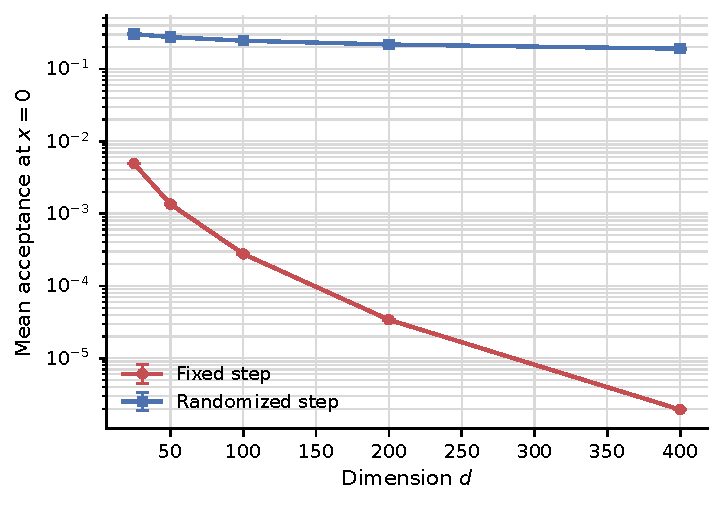
\includegraphics[width=0.72\textwidth]
		{hard_target_origin_acceptance.pdf}
		\caption{Estimated mean acceptance probability at the origin for the target
			\eqref{eq:simulation-hard-target}.  Fixed-step MALA uses \(h=h_0\), while
			randomized-step MALA uses \(h\sim\operatorname{Unif}(0,h_0)\).  The vertical
			axis is logarithmic, and vertical bars show \(\pm2\) estimated standard
			errors; most are narrower than the markers.}
		\label{fig:hard-target-origin-acceptance}
	\end{figure}
	
	As \cref{fig:hard-target-origin-acceptance} shows, the fixed-step acceptance
	probability decreases from approximately \(4.92\times10^{-3}\) at \(d=25\)
	to \(1.94\times10^{-6}\) at \(d=400\).  The randomized-step acceptance
	probability decreases much more slowly, from \(0.304\) to \(0.190\).
	Because rejection leaves a chain initialized at the origin unchanged, the
	time to its first accepted move is geometric.  At \(d=400\), the reciprocal
	acceptance estimates imply mean waiting times of approximately
	\(5.14\times10^5\) iterations for fixed-step MALA and \(5.25\) iterations
	for randomized-step MALA.  The experiment therefore directly displays the
	sticky behavior behind the fixed-step obstruction: proposals at the
	oscillation scale \(h_0\) have rapidly deteriorating acceptance, whereas
	uniform randomization retains a substantial probability of selecting a
	smaller step.
	
	
	
	To continue the origin experiment beyond one step, we next examine what
	happens after fixed-step MALA eventually escapes the hard point.  We run one
	chain of each type for \(40{,}000\) iterations on the \(d=200\) target,
	starting both chains at the origin and taking \(H=h_0\).  
	%TThe fixed chain uses
	%\(h=h_0\) throughout, whereas the randomized chain independently redraws
	%\(h\sim\operatorname{Unif}(0,h_0)\) at every iteration.  
	We record the first
	coordinate at every iteration.
	
	\begin{figure}[htbp]
		\centering
		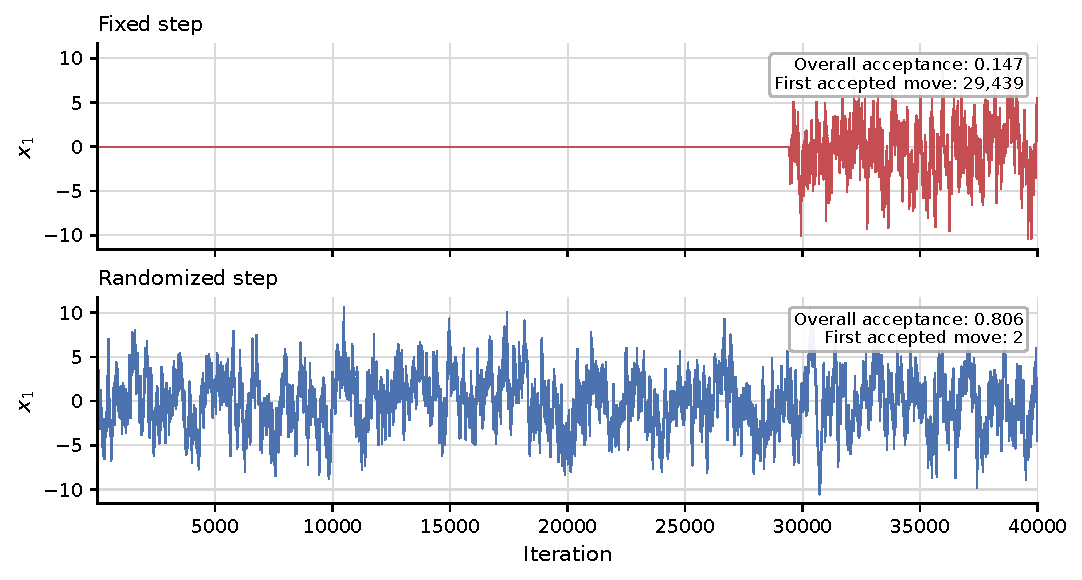
\includegraphics[width=\textwidth]
		{hard_target_first_coordinate_trace.pdf}
		\caption{First-coordinate traces continuing the origin experiment for the
			\(d=200\) hard target, with both chains initialized at the origin and
			\(H=h_0=4/\sqrt{200}\).  The two panels use common horizontal and vertical
			scales.}
		\label{fig:hard-target-first-coordinate-trace}
	\end{figure}
	
	In this realization, the fixed-step chain rejects its first \(29{,}438\)
	proposals and first moves at iteration \(29{,}439\).  It then makes
	\(5{,}882\) accepted moves by iteration \(40{,}000\), so its overall
	acceptance rate is \(0.147\).  Over the \(10{,}562\)-iteration interval from
	its first accepted move through the end of the run, its empirical acceptance
	rate is \(0.557\).  The trace therefore shows that, once the fixed chain
	escapes the sticky point, it begins moving on an ordinary scale; the low
	overall acceptance rate is dominated by the long initial wait.  The
	randomized chain first moves at iteration \(2\), makes \(32{,}253\) accepted
	moves, and has overall acceptance rate \(0.806\).
	
	
	\subsection{Stationary acceptance and jumping distance}
	
	The preceding experiment deliberately starts at an atypical point.  We next
	compare average one-step behavior under stationarity.  We fix \(d=200\) and
	\(h_0=4/\sqrt{200}\), and vary \(H/h_0\) from \(0.05\) to \(100\), using a
	fine grid near the efficient range and a logarithmically spaced grid on the
	over-tuning side.
	
	Exact stationary samples are available because
	\eqref{eq:simulation-hard-target} is a product target.  The first coordinate
	is \(N(0,m^{-1})\).  For each remaining coordinate, we propose
	\(\widetilde X\sim N(0,2/(L+m))\) and accept it with probability
	\[
	\exp\left\{
	\frac{(L-m)h_0}{2}
	\left[
	\cos\left(\frac{\widetilde X}{\sqrt{h_0}}\right)-1
	\right]
	\right\}.
	\]
	This is an exact rejection sampler.  At every endpoint~$H$ and for each method,
	we use \(48{,}000\) independent stationary one-step experiments.
	
	\begin{figure}[tbp]
		\centering
		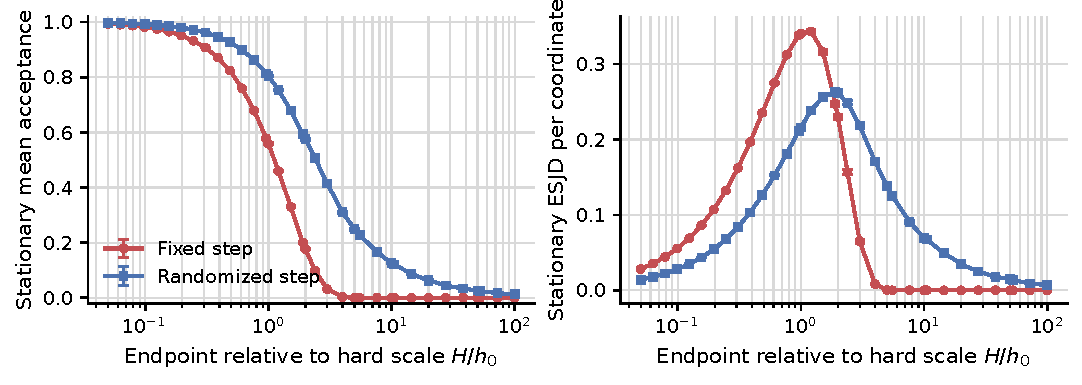
\includegraphics[width=\textwidth]
		{hard_target_stationary_comparison.pdf}
		\caption{Stationary one-step performance for the \(d=200\) target with
			\(h_0=4/\sqrt{200}\).  Fixed-step MALA uses \(h=H\), while randomized-step
			MALA uses \(h\sim\operatorname{Unif}(0,H)\).  Vertical bars show
			\(\pm2\) estimated standard errors.}
		\label{fig:hard-target-stationary}
	\end{figure}
	
	\Cref{fig:hard-target-stationary} shows the expected
	efficiency--robustness tradeoff.  At \(H=h_0\), fixed-step MALA has
	acceptance \(0.559\) and ESJD \(0.340\), while randomized-step MALA has
	acceptance \(0.804\) and ESJD \(0.216\).  The largest observed fixed-step
	ESJD is \(0.343\), at \(H/h_0\approx1.21\), whereas the largest observed
	randomized-step ESJD is \(0.263\), at \(H/h_0\approx1.90\).  Thus a
	well-tuned fixed step has the larger peak ESJD.
	
	Randomization becomes advantageous when the endpoint is too large.  
	%At
	%\(H=2h_0\), the fixed and randomized ESJDs are \(0.230\) and \(0.261\),
	%respectively.  At \(H=3h_0\), fixed-step acceptance has fallen to \(0.0316\)
	%and its ESJD to \(0.0652\), while randomized-step MALA retains acceptance
	%\(0.415\) and ESJD \(0.218\).  
	At \(H=10h_0\), fixed-step acceptance is
	extremely close to~0, whereas randomized-step MALA retains
	acceptance \(0.125\) and ESJD \(0.0692\).  Even at \(H=100 \, h_0\), the
	randomized method has acceptance \(0.0127\) and ESJD \(0.00681\), while the
	corresponding fixed-step estimates are below floating-point resolution.
	Randomization does not prevent performance from eventually decreasing as
	\(H\) grows, but it changes the abrupt fixed-step collapse into a much more
	gradual decline.
	
	The two experiments also expose a distinction relevant to the global
	spectral gap.  When \(d=200\) and \(H=h_0\), fixed-step acceptance is about
	\(0.559\) under stationarity but only \(3.40\times10^{-5}\) at the origin.
	Thus stationary-average diagnostics largely miss the small sticky region, which leads to the exceedingly small spectral gap of fixed-step MALA, as shown in \cref{app:fixed-step-obstruction}.
	Uniform randomization improves
	acceptance both in that region and under over-tuning, although it does not
	dominate a well-tuned fixed step in stationary ESJD.  These one-step
	experiments illustrate tuning robustness; they do not estimate the spectral
	gap itself.
	
	
	\bigskip
	
	\noindent{\bf Acknowledgment:} The author thanks Guanyang Wang for reading the paper and for providing helpful comments.
	
	\vspace{2cm}
	
	\noindent{\LARGE \bf Appendices}
	
	\appendix
	
	\section{Proof of Proposition~\ref{prop:minimax-fixed-step-ceiling}}
	\label{app:fixed-step-obstruction}
	
	
	We follow an
	existing line of research concerning the mixing properties of fixed-step MALA for hard target distributions.
	A perturbed-Gaussian target constructed in
	\cite[Theorems~8, 9, and~36]{ChewiEtAl2021} forms the basis of our analysis.  Subsequently,
	\citet[Equation~(28) and Lemma~8]{WuSchmidlerChen2022} combined a perturbed Gaussian block with a Gaussian coordinate, refining the construction.
	The two works do not readily yield the spectral gap upper bound in \cref{prop:minimax-fixed-step-ceiling}.
	Below, we use a modified version of the construction in \cite{WuSchmidlerChen2022} to derive the upper bound.
	
	
	\begin{proposition}
		\label{prop:generic-fixed-step-obstruction}
		There are universal constants $c,C>0$ such that the following holds.
		Let $d\geq2$, $0<m<L$, and $h>0$.  Define
		\begin{equation}
			\label{eq:generic-hard-potential}
			U_{d,h}(x)
			=\frac{m}{2}x_1^2
			+\sum_{i=2}^d\left[
			\frac{L+m}{4}x_i^2
			-\frac{(L-m)h}{2}
			\cos\left(\frac{x_i}{\sqrt h}\right)
			\right].
		\end{equation}
		Then $U_{d,h}$ is infinitely differentiable and
		\begin{equation}
			\label{eq:generic-hard-curvature}
			mI_d\preceq\nabla^2U_{d,h}(x)\preceq LI_d,
			\qquad x\in\R^d.
		\end{equation}
		If $P_h$ is the MALA kernel with step size~$h$ and target density
		proportional to $e^{-U_{d,h}}$, then
		\begin{equation}
			\label{eq:generic-fixed-step-gap-upper}
			\Gap(P_h)
			\leq
			C\min\left\{
			mh+\frac{(mh)^2}{2},
			\exp\left[
			-c(d-1)\min\{(L-m)h,1\}
			\right]
			\right\}.
		\end{equation}
		Writing $\kappa=L/m$, this further implies, after possibly changing
		the universal constants $c$ and~$C$, that
		\begin{equation}
			\label{eq:generic-fixed-step-gap-upper-kappa}
			\Gap(P_h)
			\leq
			C\min\left\{
			\kappa^{-1}Lh,
			\exp\left[
			-cd\min\{(1-\kappa^{-1})Lh,1\}
			\right]
			\right\}.
		\end{equation}
	\end{proposition}
	
	\begin{proof}
		For $i\geq2$, the $i$th diagonal entry of the Hessian of
		$U_{d,h}$ is
		\[
		\frac{L+m}{2}
		+\frac{L-m}{2}
		\cos\left(\frac{x_i}{\sqrt h}\right),
		\]
		which lies in $[m,L]$.  The first diagonal entry equals~$m$, and
		all off-diagonal entries vanish.  This proves
		\eqref{eq:generic-hard-curvature}.
		
		We first establish the local upper bound.  The target is a product
		measure, and its first marginal is $N(0,m^{-1})$.  Use
		$f(x)=x_1$ in the Poincar\'e quotient.  Let $X$ have the target
		distribution, let $Z\sim N_d(0,I_d)$ be independent of~$X$, and
		write
		\[
		\widetilde Y
		=X-h\nabla U_{d,h}(X)+\sqrt{2h}\,Z
		\]
		for the MALA proposal.  The actual transition either moves to
		$\widetilde Y$ or remains at~$X$.  Consequently,
		\begin{align*}
			\cE_{P_h}(f,f)
			&\leq
			\frac12\E\left[
			\bigl(-hmX_1+\sqrt{2h}\,Z_1\bigr)^2
			\right]\\
			&=\frac12\left(h^2m+2h\right),
		\end{align*}
		where we used $\E(X_1^2)=m^{-1}$ and the independence of
		$X_1$ and~$Z_1$.  Since $\Var_\pi(f)=m^{-1}$, it follows that
		\begin{equation}
			\label{eq:generic-local-upper}
			\Gap(P_h)
			\leq
			mh+\frac{(mh)^2}{2}.
		\end{equation}
		
		We next obtain the exponential upper bound by controlling the mean
		acceptance probability at the origin.  Write
		\[
		a=\frac{L+m}{2},
		\qquad
		b=\frac{L-m}{2}.
		\]
		At the origin, $\nabla U_{d,h}(0)=0$, so a proposal has the form
		\[
		Y=\sqrt{2h}\,Z.
		\]
		For a general differentiable potential~$U$, the log Hastings ratio
		for a proposal from $x$ to~$y$ is
		\begin{align}
			R_h(x,y)
			&:=\log
			\frac{e^{-U(y)}q_h(y,x)}
			{e^{-U(x)}q_h(x,y)}
			\notag\\
			&=U(x)-U(y)
			+\frac12
			\ip{y-x}{\nabla U(x)+\nabla U(y)}
			\notag\\
			&\quad
			+\frac h4\left[
			\norm{\nabla U(x)}^2
			-\norm{\nabla U(y)}^2
			\right].
			\label{eq:generic-log-Hastings-ratio}
		\end{align}
		For $i=2,\ldots,d$, put
		\[
		V_i=\frac{Y_i}{\sqrt h}=\sqrt2Z_i.
		\]
		Substituting \eqref{eq:generic-hard-potential} into
		\eqref{eq:generic-log-Hastings-ratio} gives
		\begin{align}
			R_h(0,Y)
			={}&-\frac{m^2h^2}{2}Z_1^2
			+bh\sum_{i=2}^d A(V_i)
			\notag\\
			&-\frac{h^2}{4}\sum_{i=2}^d
			\bigl[aV_i+b\sin(V_i)\bigr]^2,
			\label{eq:generic-hard-log-ratio}
		\end{align}
		where
		\[
		A(v)=\cos v-1+\frac{v\sin v}{2}.
		\]
		Both the first and the last terms in
		\eqref{eq:generic-hard-log-ratio} are nonpositive.
		
		Since $V_i\sim N(0,2)$,
		\[
		\E(\cos V_i)=e^{-1},
		\qquad
		\E(V_i\sin V_i)=2e^{-1}.
		\]
		The first identity follows from the characteristic function of
		$V_i$, and the second follows from Stein's identity.  Hence
		\begin{equation*}
			\E[A(V_i)]
			=\frac2e-1
			=-a_0,
			\qquad
			a_0=1-\frac2e>0.
		\end{equation*}
		Moreover,
		\[
		\abs{A(v)}\leq2+\frac{\abs v}{2}.
		\]
		Thus $A(V_i)-\E[A(V_i)]$ has a universally bounded
		sub-Gaussian norm; see, for example,
		\citep[Section~2.5.2]{Vershynin2018}.  The concentration
		inequality for sums of independent sub-Gaussian random variables
		\citep[Theorem~2.6.3]{Vershynin2018} therefore yields a universal
		constant $c_0>0$ such that
		\begin{equation}
			\label{eq:generic-hard-concentration}
			\mathbb P\left(
			\sum_{i=2}^d A(V_i)
			>-\frac{a_0(d-1)}{2}
			\right)
			\leq e^{-c_0(d-1)}.
		\end{equation}
		Outside the event in \eqref{eq:generic-hard-concentration},
		\[
		R_h(0,Y)
		\leq
		-\frac{a_0}{2}bh(d-1)
		=
		-\frac{a_0}{4}(d-1)(L-m)h.
		\]
		Let
		\[
		a_h(x)=\int\alpha_h(x,y)Q_h(x,\df y)
		\]
		denote the pointwise acceptance probability.  It follows that
		\begin{align*}
			a_h(0)
			&=\E\left[1\wedge e^{R_h(0,Y)}\right]
			\\
			&\leq
			\exp\left[
			-\frac{a_0}{4}(d-1)(L-m)h
			\right]
			+e^{-c_0(d-1)}
			\\
			&\leq
			2\exp\left[
			-c_1(d-1)\min\{(L-m)h,1\}
			\right]
		\end{align*}
		for a universal constant $c_1>0$.
		
		The function $x\mapsto a_h(x)$ is continuous.  Indeed, writing
		the proposal as
		\[
		x-h\nabla U_{d,h}(x)+\sqrt{2h}\,Z,
		\qquad Z\sim N_d(0,I_d),
		\]
		the resulting acceptance probability is continuous in~$x$ for
		every fixed~$Z$ and is bounded by one.  Continuity therefore
		follows from dominated convergence.
		
		Consequently, there is an open ball~$S$ centered at the origin
		such that
		\[
		0<\pi(S)\leq\frac12,
		\qquad
		\sup_{x\in S}a_h(x)
		\leq
		4\exp\left[
		-c_1(d-1)\min\{(L-m)h,1\}
		\right].
		\]
		A transition starting in~$S$ can leave~$S$ only if its proposal
		is accepted.  Hence
		\[
		\mathcal{J}_{P_h}(S,S^c)
		\leq
		4\exp\left[
		-c_1(d-1)\min\{(L-m)h,1\}
		\right]\pi(S).
		\]
		Testing the Poincar\'e quotient with $\mathbf 1_S$ gives
		\begin{align}
			\Gap(P_h)
			&\leq
			\frac{\cE_{P_h}(\mathbf 1_S,\mathbf 1_S)}
			{\Var_\pi(\mathbf 1_S)}
			\notag\\
			&=
			\frac{\mathcal{J}_{P_h}(S,S^c)}
			{\pi(S)[1-\pi(S)]}
			\notag\\
			&\leq
			8\exp\left[
			-c_1(d-1)\min\{(L-m)h,1\}
			\right].
			\label{eq:generic-hard-sticky-gap}
		\end{align}
		Combining \eqref{eq:generic-local-upper} and
		\eqref{eq:generic-hard-sticky-gap} proves
		\eqref{eq:generic-fixed-step-gap-upper}.
		
		Finally, we prove
		\eqref{eq:generic-fixed-step-gap-upper-kappa}.  We have
		\[
		L-m=(1-\kappa^{-1})L,
		\qquad
		d-1\geq\frac d2.
		\]
		Therefore
		\[
		(d-1)\min\{(L-m)h,1\}
		\geq
		\frac d2
		\min\{(1-\kappa^{-1})Lh,1\}.
		\]
		If $mh\leq1$, then
		\[
		mh+\frac{(mh)^2}{2}
		\leq\frac32mh
		=\frac32\kappa^{-1}Lh.
		\]
		If $mh>1$, then
		\[
		\exp\left[
		-cd\min\{(1-\kappa^{-1})Lh,1\}
		\right]
		\leq1<mh=\kappa^{-1}Lh,
		\]
		so the exponential bound is the smaller of the two terms in
		\eqref{eq:generic-fixed-step-gap-upper-kappa}.  After adjusting
		the universal constants, this proves
		\eqref{eq:generic-fixed-step-gap-upper-kappa}.
	\end{proof}
	
	
	
	We can now prove \cref{prop:minimax-fixed-step-ceiling}.
	
	\begin{proof}
		By \cref{prop:generic-fixed-step-obstruction}, there are universal
		constants $c_0,C_0>0$ such that, for every $h>0$,
		\begin{equation}
			\label{eq:minimax-two-branches}
			\inf_{\substack{U\in C^\infty(\R^d)\\
					mI_d\preceq\nabla^2U(x)\preceq LI_d,\ x\in\R^d}}
			\Gap(P_{U,h})
			\leq F(Lh),
		\end{equation}
		where
		\[
		F(t)
		=
		C_0\min\left\{
		\kappa^{-1}t,\,
		\exp\left[
		-c_0d\min\{(1-\kappa^{-1})t,1\}
		\right]
		\right\}.
		\]
		Set
		\[
		t_\star
		=
		\frac{2\log(\kappa d)}
		{c_0(1-\kappa^{-1})d}.
		\]
		If $0<t\leq t_\star$, then
		\[
		F(t)
		\leq
		C_0\kappa^{-1}t_\star
		=
		\frac{2C_0\log(\kappa d)}
		{c_0(1-\kappa^{-1})\kappa d}.
		\]
		If $t>t_\star$, then the exponential term defining $F$ is
		nonincreasing in~$t$, and hence
		\begin{align*}
			F(t)
			&\leq
			C_0\exp\left[
			-c_0d\min\{(1-\kappa^{-1})t_\star,1\}
			\right]\\
			&=
			C_0\max\left\{
			\frac{1}{(\kappa d)^2},
			e^{-c_0d}
			\right\}.
		\end{align*}
		Consequently,
		\begin{equation}\label{eq:minimax-F-upper}
			\begin{aligned}
				\sup_{t>0}F(t)
				&\leq
				C_0\max\left\{
				\frac{2\log(\kappa d)}
				{c_0(1-\kappa^{-1})\kappa d},
				\frac{1}{(\kappa d)^2},
				e^{-c_0d}
				\right\} \\
				&\leq C_0\max\left\{
				\frac{2\log(\kappa d)}
				{c_0(1-\kappa_0^{-1})\kappa d},
				\frac{1}{(\kappa d)^2},
				e^{-c_0d}
				\right\}.
			\end{aligned}
		\end{equation}
		Because $d\geq2$ and $\kappa>1$,
		\[
		\frac{1}{(\kappa d)^2}
		\leq
		C\frac{\log(\kappa d)}{\kappa d}
		\]
		for a universal constant~$C$.  Absorbing the factors depending
		only on $\kappa_0$ into~$C$, and changing the universal
		exponential constant if necessary, \eqref{eq:minimax-two-branches} and \eqref{eq:minimax-F-upper}
		prove \eqref{eq:minimax-fixed-step-ceiling}.
	\end{proof}
	
	
	
	
	
	\section{Proof of Proposition~\ref{prop:overlap}}\label{app:rejection-overlap}
	
	This appendix proves \cref{prop:overlap}.
	The convexity assumption on \(U\) is not needed for
	\cref{prop:stationary-rejection,lem:linear-increment,lem:integrated-increments,lem:frozen-endpoint-law,lem:path-likelihood}.
	For these results it suffices that \(U\in C^1(\R^d)\), that
	\(\nabla U\) be globally \(L\)-Lipschitz for some \(L>0\), and that
	\(0<\int_{\R^d}e^{-U(x)}\,\df x<\infty\), with \(\pi\) the normalized
	measure and \(X_0\sim\pi\). Under these weaker assumptions the Langevin
	diffusion is still nonexplosive and reversible with respect to \(\pi\);
	see \citet[Section~2, assumption~L1 and the subsequent discussion]{DurmusMoulines2017}.
	The proofs of the stated results below use only these weaker assumptions.
	The globally safe assertion of \cref{prop:overlap}, proved at the end of
	this appendix, continues to use convexity.
	
	The main input is the following stationary estimate for the pointwise rejection function
	\[
	r_h(x)=1-\int\alpha_h(x,y)Q_h(x,\df y),
	\]
	where
	\[
	\alpha_h(x,y)
	=1\wedge
	\frac{e^{-U(y)}q_h(y,x)}{e^{-U(x)}q_h(x,y)},
	\qquad
	q_h(x,y)=(4\pi h)^{-d/2}
	\exp\left\{-\frac{\norm{y-x+h\nabla U(x)}^2}{4h}\right\}.
	\]
	
	
	\begin{proposition} \label{prop:stationary-rejection}
		There are universal constants \(c,C>0\) such that, for every real
		\(p\geq 1\),
		\begin{equation}\label{eq:stationary-rejection}
			h\leq\frac{c}{L\sqrt{p(d+p)}}
			\quad\Longrightarrow\quad
			\norm{r_h}_{L^p(\pi)}
			\leq
			CLh\sqrt{p(d+p)}.
		\end{equation}
	\end{proposition}
	
	The proof of \cref{prop:stationary-rejection} compares the exact stationary Langevin path with the path whose
	drift is frozen at its initial position.  The endpoint of the latter path
	is exactly the MALA proposal.  Similar diffusion-comparison ideas appear in
	\citet{BouRabeeVandenEijnden2010,BouRabeeHairer2013,ChewiEtAl2021}.
	
	The idea behind the proof is roughly as follows.
	Let $X_0 \sim \pi$, and suppose that, on a filtered probability space $(\Omega,\mathcal F,(\mathcal F_t)_{t\geq0},\mathbb P)$, $X_t$ solves the Langevin equation
	\begin{equation} \label{eq:langevin}
		\df X_t = -\nabla U(X_t) \, \df t + \sqrt{2} \df B_t,
	\end{equation}
	where $B_t$ is a Brownian motion.
	Standard theory of Langevin diffusion implies $X_h \sim \pi$.
	Denote by $S_h$ the conditional distribution of $X_h$ given $X_0$.
	We compare $S_h(x, \df y)$ to the proposal $Q_h(x, \df y)$, which gives the Gaussian law $N_d(x - h \nabla U(x), 2h I_d)$.
	Define $\nu_h(\df x, \df y) = \pi(\df x) S_h(x, \df y)$, $\mu_h(\df x, \df y) = \pi(\df x) Q_h(x, \df y)$.
	Assume that the Radon-Nikodym derivative $F_h = \df \mu_h/\df \nu_h$ can be found.
	Since the Langevin diffusion is $\pi$-reversible, it holds that $\nu_h$ is symmetric, and
	\[
	\frac{\df \mu_h^{\top}}{\df \mu_h}(x,y) = \frac{F_h(y,x)}{F_h(x,y)},
	\]
	where $\mu_h^{\top}(\df x, \df y) = \mu_h(\df y, \df x)$.
	Moreover, it can be argued that, for $\pi$-a.e. $x$, $F_h(x, \cdot) = \df Q_h(x,\cdot)/\df S_h(x,\cdot)$.
	Then
	\[
	\begin{aligned}
		r_h(x) &= \int S_h(x, \df y) \left[ 1 - F_h(x,y) \min\left\{ 1, \frac{F_h(y,x)}{F_h(x,y)} \right\} \right]  \\
		&\leq \int(|F_h(x,y) - 1| + |F_h(y,x) - 1|) \, S_h(x, \df y).
	\end{aligned}
	\]
	Using Jensen's inequality and the fact that $\nu_h$ is symmetric, one can now show that $\|r_h\|_{L^p(\pi)}$ can be controlled by $2 \|F_h - 1\|_{L^p(\nu_h)}$.
	
	To find $F_h$, let 
	\[
	\df W_t = \df B_t - \theta_t \, \df t, \quad \theta_t = \frac{\nabla U(X_t) - \nabla U(X_0)}{\sqrt{2}}
	\]
	Then $X_t$ has the frozen drift representation $\df X_t = - \nabla U(X_0) \df t + \sqrt{2} \df W_t$.
	Suppose that one can find an alternative probability measure $\mathbb P_h^{\mathrm{fr}}$ defined by a Radon-Nikodym derivative $D_h = \df \mathbb P_h^{\mathrm{fr}}/\df \mathbb P|_{\mathcal{F}_h}$ such that, under $\mathbb P_h^{\mathrm{fr}}$, $W_t$ is a Brownian motion with respect to $(\mathcal{F}_t)_{0 \leq t \leq h}$.
	Then, under this new probability measure, $(X_0, X_h)$ is distributed as $\mu_h$.
	In particular, with expectations defined in terms of $\mathbb{P}$, $F_h(X_0, X_h) = \mathbb{E}[D_h \mid \sigma(X_0, X_h)]$, so conditional Jensen's inequality would imply that $\|F_h - 1\|_{L^p(\nu_h)} \leq \|D_h - 1\|_{L^p(\mathbb{P})}$.
	As stated in \cref{lem:frozen-endpoint-law}, one can construct the desired measure $\mathbb{P}_h^{\mathrm{fr}}$ by letting $D_h$ be defined through the stochastic exponential
	\[
	D_t = \exp\left( \int_0^t \langle \theta_s, \df B_s \rangle - \frac{1}{2} V_t \right), \quad V_t = \int_0^t \|\theta_s\|^2 \, \df s,
	\]
	provided that $(D_t)_{0 \leq t \leq h}$ is a true martingale.
	This is a consequence of  Girsanov's theorem \citep[see, e.g.,][]{KaratzasShreve1991,RevuzYor1999}.
	Therefore, to prove \cref{prop:stationary-rejection}, it comes down to two tasks: showing that $D_t$ is a true martingale, and that $\|D_h - 1\|_{L^p(\mathbb{P})} \leq C L h \sqrt{p(d+p)}$ when $h \leq c/(L\sqrt{p(d+p)})$, where $c, C$ are appropriate universal constants.
	
	To show that $D_t$ is a martingale, it suffices to establish Novikov's criterion: $\mathbb{E} (e^{V_h/2}) < \infty$.
	Since $\nabla U$ is $L$-Lipschitz, one can bound $V_h$ by $L^2 J_h/2$, where $J_h = \int_0^h \|X_t - X_0\|^2 \, \df t$.
	This prompts us to bound $\mathbb{E}(e^{\lambda J_h})$ for some suitable $\lambda \geq 0$ in \cref{lem:integrated-increments}.
	
	We obtain the upper bound $\|D_h - 1\|_{L^p(\mathbb{P})} \leq C L h \sqrt{p(d+p)}$ for $h \leq c/(L\sqrt{p(d+p)})$ in \cref{lem:path-likelihood}.
	In the proof of \cref{lem:path-likelihood}, we apply It\^o's formula, Burkholder-Davis-Gundy (BDG) inequality, and Doob's maximal inequality to obtain what is loosely
	\[
	\|D_h - 1\|_{L^p(\mathbb{P})} \leq C' \sqrt{p} \, \|V_h\|_{L^p(\mathbb{P})}^{1/2} \leq 2^{-1/2} C' L \sqrt{p} \, \|J_h\|_{L^p(\mathbb{P})}^{1/2},
	\]
	where $C'$ is universal.
	This prompts us to study $\|J_h\|_{L^p(\mathbb{P})}$ and obtain an upper bound that is of order $h^2(d+p)$ in \cref{lem:integrated-increments}.
	
	To establish the bounds in \cref{lem:integrated-increments}, we first
	control \(X_t-X_0\) using stationary reversibility in
	\cref{lem:linear-increment}, without explicitly solving the
	Langevin equation.
	
	
	Once \cref{prop:stationary-rejection} is established, we can utilize elementary techniques in the MCMC literature \citep[see, e.g.,][proof of Theorem~3]{WuSchmidlerChen2022} to establish \cref{prop:overlap}.
	
	\paragraph{Attribution within this appendix.}
	The estimate in \cref{lem:linear-increment} is an elementary consequence
	of the Lyons--Zheng forward--backward decomposition
	\citep[Section~1, especially equation~(1.7)]{LyonsZheng1988}; see also
	\citet[Theorem~5.7.1]{FukushimaOshimaTakeda2011}.
	For the Langevin diffusion considered here, the required decomposition
	follows directly from the stochastic differential equation and stationary
	reversibility, as shown below.
	\cref{lem:integrated-increments} then follows from that estimate,
	Gaussian randomization, and Jensen's inequality.
	The Gaussian-randomization step is the identity-matrix specialization
	of the argument used for sub-Gaussian quadratic forms by
	\citet[Theorem~1 and Remark~2]{HsuKakadeZhang2012}.
	\cref{lem:path-likelihood} combines standard results on stochastic
	exponentials, Novikov's criterion, Girsanov's theorem, stopping of
	stochastic integrals, Doob's inequality, and the quantitative BDG
	inequality, with the problem-specific estimate \(V_h\leq L^2J_h/2\).
	General reverse-H\"older theory for continuous stochastic exponentials
	is developed by \citet{Kazamaki1994}, but the dimension- and
	moment-explicit calculation needed here is supplied in full.
	The passage from the path likelihood to the rejection probability uses
	the standard conditional-likelihood identity and the
	Metropolis--Hastings meet identity
	\citep{Kallenberg2021,Tierney1998,BilleraDiaconis2001}.
	Thus \cref{prop:stationary-rejection} combines these ingredients for
	the present MALA problem.
	
	\subsection{Controlling Langevin increments}
	
	The goal of this subsection is to control the magnitude of \(X_t-X_0\),
	particularly the time integral
	\(\int_0^h\norm{X_t-X_0}^2\,\df t\), where \(X_t\) satisfies
	\eqref{eq:langevin}.
	
	We begin by fixing the continuous-time framework used throughout this
	appendix. All random variables are defined on a filtered probability
	space
	\[
	(\Omega,\mathcal F,(\mathcal F_t)_{t\geq0},\mathbb P)
	\]
	satisfying the usual completeness and right-continuity conditions.
	A standard \(d\)-dimensional Brownian motion relative to this filtration
	is an adapted continuous process \(B\) with \(B_0=0\) such that, for
	\(0\leq s<t\), the increment \(B_t-B_s\) has law
	\(N_d(0,(t-s)I_d)\) and is independent of \(\mathcal F_s\).
	This last independence property will be used explicitly in
	\cref{ssec:girsanov-frozen}.
	Basic references for filtered probability spaces, Brownian motion,
	It\^o integration, and stochastic differential equations are
	\citet[Chapters~3 and~5]{KaratzasShreve1991},
	\citet[Chapters~IV and~IX]{RevuzYor1999}, and
	\citet{Kallenberg2021}.
	
	Because \(\nabla U\) is globally Lipschitz, for every \(x\in\R^d\)
	the Langevin equation has a unique nonexplosive strong solution
	\((X_t^x)_{t\geq0}\) with \(X_0^x=x\); see, for example,
	\citet[Chapter~5]{KaratzasShreve1991}.
	For a bounded measurable function \(f\), define the transition
	semigroup by
	\[
	S_tf(x)=\E[f(X_t^x)].
	\]
	
	Now let \(X_0\) be \(\mathcal F_0\)-measurable and independent of \(B\),
	with law \(\pi\), and let \((X_t)_{t\geq0}\) be the corresponding
	solution of
	\begin{equation}\label{eq:langevin-sde}
		\df X_t=-\nabla U(X_t)\,\df t+\sqrt{2}\,\df B_t,
		\qquad X_0\sim\pi.
	\end{equation}
	The differential notation means the integral identity
	\begin{equation}\label{eq:langevin-integral}
		X_t=X_0-\int_0^t\nabla U(X_s)\,\df s+\sqrt{2}\,B_t,
		\qquad t\geq0.
	\end{equation}
	Under the weaker assumptions stated at the beginning of this appendix,
	the Langevin semigroup is symmetric with respect to
	\(\pi(\df x)\propto e^{-U(x)}\,\df x\):
	\[
	\int fS_tg\,\df\pi=\int gS_tf\,\df\pi
	\]
	for bounded measurable \(f,g\) and \(t\geq0\); see
	\citet[Section~2]{DurmusMoulines2017} and
	\citet[Chapters~1 and~7]{FukushimaOshimaTakeda2011}.
	Since \(S_t1=1\), taking \(f=1\) shows that \(\pi\) is invariant.
	Consequently, the process started from \(X_0\sim\pi\) is stationary
	and reversible.
	
	\begin{lemma}\label{lem:linear-increment}
		For every \(v\in\R^d\), \(\lambda\in\R\), and \(t\geq0\),
		\begin{equation}\label{eq:linear-increment-mgf}
			\E[\exp(\lambda\ip{v}{X_t-X_0})]
			\leq
			\exp(\lambda^2t\norm{v}^2).
		\end{equation}
	\end{lemma}
	
	\begin{proof}
		The case \(t=0\) is immediate. Fix \(t>0\).
		Stationarity and reversibility give
		\[
		(X_s)_{0\leq s\leq t}
		\stackrel{\mathrm d}{=}
		(X_{t-s})_{0\leq s\leq t}
		\]
		as random elements of \(C([0,t];\R^d)\).
		Set
		\[
		Z_t=X_0-X_t+\int_0^t\nabla U(X_s)\,\df s.
		\]
		Reversing the path interchanges \(X_0\) and \(X_t\), while leaving
		the time integral unchanged, since
		\[
		\int_0^t\nabla U(X_{t-s})\,\df s
		=
		\int_0^t\nabla U(X_s)\,\df s.
		\]
		The equality of path laws and \eqref{eq:langevin-integral} therefore give
		\[
		Z_t
		\stackrel{\mathrm d}{=}
		X_t-X_0+\int_0^t\nabla U(X_s)\,\df s
		=
		\sqrt{2}\,B_t
		\sim N_d(0,2tI_d).
		\]
		Moreover, subtracting the definition of \(Z_t\) from the preceding
		expression for \(\sqrt{2}\,B_t\) yields
		\[
		X_t-X_0=\frac{\sqrt{2}\,B_t-Z_t}{2}.
		\]
		Thus the drift integral cancels when the forward and reversed
		expressions are subtracted.
		
		By convexity of the exponential function,
		\begin{align*}
			\E[\exp(\lambda\ip{v}{X_t-X_0})]
			&=
			\E\left[
			\exp\left(\frac{\lambda}{2}
			\ip{v}{\sqrt{2}\,B_t-Z_t}\right)
			\right]\\
			&\leq
			\frac12\E[\exp(\sqrt{2}\lambda\ip{v}{B_t})]
			+
			\frac12\E[\exp(-\lambda\ip{v}{Z_t})]\\
			&=
			\exp(\lambda^2t\norm{v}^2).
		\end{align*}
		The last equality uses the Gaussian moment-generating formula.
		No independence between \(B_t\) and \(Z_t\) is required, and the
		finite Gaussian exponential moments justify the inequality without
		any preliminary integrability assumption on its left-hand side.
	\end{proof}
	
	The next proof uses a standard Gaussian-randomization argument.  In a more
	general matrix form, it is the argument used by
	\citet[Theorem~1 and Remark~2]{HsuKakadeZhang2012} to pass from linear
	sub-Gaussian moment bounds to quadratic-form bounds.  We include the
	identity-matrix calculation because the exact constant in
	\eqref{eq:quadratic-increment-mgf} is useful below.
	
	\begin{lemma} \label{lem:integrated-increments}
		For every \(t>0\) and \(0\leq a<1/(4t)\),
		\begin{equation}\label{eq:quadratic-increment-mgf}
			\E[\exp(a\norm{X_t-X_0}^2)]
			\leq
			(1-4at)^{-d/2}.
		\end{equation}
		If
		\[
		J_h=\int_0^h\norm{X_t-X_0}^2\,\df t,
		\]
		then, for \(0\leq\lambda<1/(4h^2)\),
		\begin{equation}\label{eq:Jh-mgf}
			\E (e^{\lambda J_h})
			\leq
			(1-4\lambda h^2)^{-d/2}.
		\end{equation}
		Consequently, for every real \(p\geq1\),
		\begin{equation}\label{eq:Jh-moment}
			\norm{J_h}_{L^p(\mathbb P)}
			\leq
			C h^2(d+p),
		\end{equation}
		where \(C\) is universal.
	\end{lemma}
	
	\begin{proof}
		Enlarge the probability space,
		if necessary, so that it also carries a random vector
		\(G\sim N_d(0,I_d)\) independent of the entire Langevin path
		\((X_s)_{s\geq0}\).  For a fixed vector \(z\in\R^d\), the scalar
		\(\ip{G}{z}\) is Gaussian with mean zero and variance \(\norm{z}^2\).
		The Gaussian moment-generating formula therefore gives
		\begin{equation*}
			\E\!
			\left(
			e^{\sqrt{2a}\ip{G}{z}}
			\right)
			=e^{a\norm{z}^2}.
		\end{equation*}
		Apply this identity with the random vector \(z=X_t-X_0\).  More precisely,
		conditioning first on the Langevin path gives
		\begin{align*}
			\E \left(e^{a\norm{X_t-X_0}^2} \right)
			&=\E\left\{
			\E\left[
			e^{\sqrt{2a}\ip{G}{X_t-X_0}}
			\mathrel{\big|}\sigma(X_s:s\geq0)
			\right]
			\right\}.
		\end{align*}
		The integrand is nonnegative, so Tonelli's theorem allows us to reverse the
		order in which the path and \(G\) are averaged.  Conditional on \(G\), the
		vector \(G\) is fixed, and \cref{lem:linear-increment}, with
		\(v=G\) and \(\lambda=\sqrt{2a}\), gives
		\[
		\E\left(
		e^{\sqrt{2a}\ip{G}{X_t-X_0}}
		\mathrel{\big|}G
		\right)
		\leq e^{2at\norm{G}^2}.
		\]
		Consequently,
		\begin{equation*}
			\begin{aligned}
				\E \left(e^{a\norm{X_t-X_0}^2} \right)
				&\leq \E \left(e^{2at\norm{G}^2} \right)\\
				&=(1-4at)^{-d/2},
			\end{aligned}
		\end{equation*}
		where the last equality is the moment-generating function of a
		\(\chi_d^2\) random variable and requires \(4at<1\).  This proves
		\eqref{eq:quadratic-increment-mgf}.
		
		We next pass from one increment to its time integral.  For each fixed sample
		path, Jensen's inequality for the convex function \(x\mapsto e^x\), applied
		to the uniform probability measure \(\df t/h\) on \([0,h]\), gives
		\begin{align*}
			e^{\lambda J_h}
			&=\exp\left(
			\frac1h\int_0^h \lambda h\norm{X_t-X_0}^2\,\df t
			\right)\\
			&\leq
			\frac1h\int_0^h
			e^{\lambda h\norm{X_t-X_0}^2}\,\df t.
		\end{align*}
		Take expectations and use Tonelli's theorem, followed by
		\eqref{eq:quadratic-increment-mgf} with \(a=\lambda h\):
		\begin{align*}
			\E (e^{\lambda J_h})
			&\leq
			\frac1h\int_0^h
			\E (e^{\lambda h\norm{X_t-X_0}^2}) \,\df t\\
			&\leq
			\frac1h\int_0^h(1-4\lambda ht)^{-d/2}\,\df t\\
			&\leq(1-4\lambda h^2)^{-d/2}.
		\end{align*}
		This proves \eqref{eq:Jh-mgf}.
		
		It remains to derive the \(L^p\) estimate from this exponential-tail bound.
		Put \(\lambda=(8h^2)^{-1}\) in
		\eqref{eq:Jh-mgf}.  Markov's inequality gives, for every \(s\geq0\),
		\begin{equation*}
			\mathbb P\left(
			J_h\geq4dh^2\log 2+8h^2s
			\right)
			\leq e^{-s}.
		\end{equation*}
		Define
		\[
		Y=\frac{(J_h-4dh^2\log 2)_+}{8h^2}.
		\]
		Then \(\mathbb P(Y>s)\leq e^{-s}\).  For every real \(p\geq1\), the
		layer-cake formula for moments gives
		\begin{align*}
			\E (Y^p)
			&=p\int_0^\infty s^{p-1}\mathbb P(Y>s)\,\df s\\
			&\leq p\int_0^\infty s^{p-1}e^{-s}\,\df s
			=\Gamma(p+1).
		\end{align*}
		Stirling's bound implies \(\Gamma(p+1)^{1/p}\leq Cp\) for all
		\(p\geq1\).  Hence, by the Minkowski inequality,
		\[
		\norm{J_h}_{L^p(\mathbb P)}
		\leq4dh^2\log 2+8h^2\norm{Y}_{L^p(\mathbb P)}
		\leq Ch^2(d+p),
		\]
		which proves \eqref{eq:Jh-moment}.  For the tail-integration identity and the
		Gamma-function estimate, see
		\citet[Chapter~2]{BoucheronLugosiMassart2013}.
	\end{proof}
	
	\subsection{Girsanov comparison with frozen drift}\label{ssec:girsanov-frozen}
	
	We compare two laws on the same path space over \([0,h]\).  Under the
	probability measure \(\mathbb P\), the path satisfies the exact
	Langevin equation \eqref{eq:langevin-sde}.  We shall construct a second
	measure under which the coordinate process has drift frozen at the initial
	value \(-\nabla U(X_0)\).
	
	We recall the continuous-martingale facts used below.  If \(H_t\) is a
	predictable \(\R^d\)-valued process with
	\(\int_0^h\norm{H_t}^2\,\df t<\infty\) almost surely, then
	\(\int_0^t\ip{H_s}{\df B_s}\) is a continuous local martingale.  Its quadratic
	variation is
	\[
	\left[
	\int_0^\cdot\ip{H_s}{\df B_s}
	\right]_t
	=\int_0^t\norm{H_s}^2\,\df s.
	\]
	For a continuous
	local martingale \(N\) with \(N_0=0\), the stochastic exponential is
	\[
	\mathcal E(N)_t=\exp(N_t-[N]_t/2).
	\]
	It is always a nonnegative local martingale, but it need not have expectation
	one.  Novikov's criterion states that
	\(\E\exp([N]_h/2)<\infty\) is sufficient for
	\((\mathcal E(N)_t)_{0\leq t\leq h}\) to be a true mean-one martingale.
	These statements, together with It\^o's formula and the stopping arguments
	used below, are standard; see \citet[Chapter~3]{KaratzasShreve1991},
	\citet[Chapters~IV and~VIII]{RevuzYor1999}, or
	\citet{Kallenberg2021}.
	
	Define
	\begin{equation*}
		\theta_t=
		\frac{\nabla U(X_t)-\nabla U(X_0)}{\sqrt{2}},
		\qquad
		V_t=\int_0^t\norm{\theta_s}^2\,\df s,
		\qquad
		M_t=\int_0^t\ip{\theta_s}{\df B_s}.
	\end{equation*}
	The process \(\theta_t\) is continuous and adapted, hence predictable.  Since
	\(X\) has continuous paths, \(\int_0^h\norm{\theta_s}^2\,\df s<\infty\) almost
	surely on every finite interval, so the It\^o integral is well defined as a
	continuous local \(\mathbb P\)-martingale.  Its quadratic variation is
	\([M]_t=V_t\).  The Lipschitz property of \(\nabla U\) and
	\cref{lem:integrated-increments} give
	\begin{equation}\label{eq:V-J}
		V_h
		\leq
		\frac{L^2}{2}J_h,
		\qquad
		\norm{V_h}_{L^p(\mathbb P)}
		\leq
		C L^2h^2(d+p)
		\; \text{whenever }p\geq1.
	\end{equation}
	Define the stochastic exponential
	\begin{equation*}
		D_t=\exp\left( M_t-\frac12V_t\right) = \mathcal E(M)_t.
	\end{equation*}
	
	The following lemma collects the change-of-measure construction and the
	endpoint identification that will be used in the proof of
	\cref{prop:stationary-rejection}.
	
	\begin{lemma}
		\label{lem:frozen-endpoint-law}
		Assume that \(h>0\) and \(Lh<1\).  Then
		\((D_t)_{0\leq t\leq h}\) is a true mean-one \(\mathbb P\)-martingale, and
		\begin{equation}\label{eq:frozen-measure-definition}
			\frac{\df\mathbb P_h^{\mathrm{fr}}}{\df\mathbb P}
			\bigg|_{\mathcal F_h}=D_h
		\end{equation}
		defines a probability measure \(\mathbb P_h^{\mathrm{fr}}\) on \((\Omega,\mathcal F_h)\).  Under
		\(\mathbb P_h^{\mathrm{fr}}\), the process
		\[
		W_t=B_t-\int_0^t\theta_s\,\df s,
		\qquad 0\leq t\leq h,
		\]
		is a Brownian motion relative to
		\((\mathcal F_t)_{0\leq t\leq h}\), and
		\begin{equation}\label{eq:frozen-path}
			X_t=X_0-t\nabla U(X_0)+\sqrt{2}\,W_t,
			\qquad 0\leq t\leq h.
		\end{equation}
		Moreover, under \(\mathbb P_h^{\mathrm{fr}}\), \(X_0\sim\pi\), and a version
		of the conditional law of \(X_h\) given \(X_0=x\) is \(Q_h(x,\cdot)\).
		It follows that, for all Borel sets \(A,B\subseteq\R^d\),
		\begin{equation}\label{eq:frozen-endpoint-law}
			\mathbb P_h^{\mathrm{fr}}(X_0\in A,X_h\in B)
			=\int_A Q_h(x,B)\,\pi(\df x).
		\end{equation}
	\end{lemma}
	
	\begin{proof}
		By \eqref{eq:Jh-mgf} and \eqref{eq:V-J},
		\begin{align*}
			\E\left[\exp\left([M]_h/2\right)\right]
			&=\E\left[\exp\left(V_h/2\right)\right]\\
			&\leq\E\left[\exp\left(L^2J_h/4\right)\right]\\
			&\leq(1-L^2h^2)^{-d/2}<\infty,
		\end{align*}
		where the last inequality uses \(Lh<1\).  Novikov's criterion therefore
		shows that \(D\) is a true mean-one \(\mathbb P\)-martingale.  In
		particular,
		\begin{equation}\label{eq:D-conditional-martingale}
			\E(D_t\mid\mathcal F_s)=D_s,
			\qquad 0\leq s\leq t\leq h,
		\end{equation}
		and \eqref{eq:frozen-measure-definition} defines a probability measure.
		
		Girsanov's theorem gives the asserted Brownian motion \(W_t\); see
		\citet[Section~3.5]{KaratzasShreve1991} or
		\citet[Chapter~VIII, Section~1]{RevuzYor1999}.  Substituting
		\[
		B_t=W_t+\int_0^t\theta_s\,\df s
		\]
		into \eqref{eq:langevin-integral} yields
		\begin{align*}
			X_t
			&=X_0-\int_0^t\nabla U(X_s)\,\df s
			+\sqrt{2}\,W_t
			+\sqrt{2}\int_0^t\theta_s\,\df s\\
			&=X_0-t\nabla U(X_0)+\sqrt{2}\,W_t,
		\end{align*}
		which proves \eqref{eq:frozen-path}.
		
		For every Borel set \(A\subseteq\R^d\),
		\begin{align*}
			\mathbb P_h^{\mathrm{fr}}(X_0\in A)
			&=\E\left(D_h\1_{\{X_0\in A\}}\right)\\
			&=\E\left[
			\E(D_h\mid\mathcal F_0)\1_{\{X_0\in A\}}
			\right]\\
			&=\mathbb P(X_0\in A)
			=\pi(A),
		\end{align*}
		where \eqref{eq:D-conditional-martingale} gives
		\(\E[D_h\mid\mathcal F_0]=D_0=1\).
		
		Under \(\mathbb P_h^{\mathrm{fr}}\), the increment \(W_h-W_0=W_h\) is
		independent of \(\mathcal F_0\) and has law \(N_d(0,hI_d)\).  Since \(X_0\)
		is \(\mathcal F_0\)-measurable, \eqref{eq:frozen-path} gives, conditionally
		on \(X_0=x\),
		\[
		X_h=x-h\nabla U(x)+\sqrt{2h}\,Z,
		\qquad Z\sim N_d(0,I_d).
		\]
		This is precisely the kernel \(Q_h(x,\cdot)\).  Combining this conditional
		law with \(X_0\sim\pi\) proves \eqref{eq:frozen-endpoint-law}.
	\end{proof}
	
	We next quantify how close the path likelihood \(D_h\) is to one.
	General reverse-H\"older and moment estimates for continuous stochastic
	exponentials form a classical theory; see, for example,
	\citet[Chapters~1 and~3]{Kazamaki1994}.  We give a direct localized
	calculation to track explicitly the dependence on $d,p,L$, and $h$ and to
	exploit the problem-specific bound $V_h\leq L^2J_h/2$.
	
	\begin{lemma}\label{lem:path-likelihood}
		There are universal constants \(c,C>0\) such that, for every \(h>0\) and
		every real \(p\geq 1\), the conditions
		\begin{equation}\label{eq:D-moment-condition}
			Lh<1,
			\qquad
			h\leq\frac{c}{L\sqrt{p(d+p)}}
		\end{equation}
		imply
		\begin{equation}\label{eq:D-moments}
			\norm{D_h}_{L^{2p}(\mathbb P)}\leq C,
			\qquad
			\norm{D_h-1}_{L^p(\mathbb P)}
			\leq CLh\sqrt{p(d+p)}.
		\end{equation}
	\end{lemma}
	
	\begin{proof}
		\noindent {\it Stopping conventions.}
		We use standard process-level stopping identities. If \(N_t\) is a continuous local martingale and
		\(\tau\) is a stopping time, then, up to indistinguishability,
		\begin{equation} \label{eq:quadratic-stop}
			N_t^\tau:=N_{t\wedge\tau},
			\qquad
			[N^\tau]_t=[N]_{t\wedge\tau}.
		\end{equation}
		Likewise, for a predictable integrand \(H_t\),
		\begin{equation}\label{eq:stopped-stochastic-integral}
			\left(\int_0^\cdot\ip{H_s}{\df B_s}\right)_{t\wedge\tau}
			=
			\int_0^t\1_{\{s\leq\tau\}}\ip{H_s}{\df B_s}.
		\end{equation}
		%	In particular, if
		%	\(\mathcal E(N)_t=\exp\left(N_t-[N]_t/2\right)\) denotes the stochastic
		%	exponential, then
		%	\[
		%	\mathcal E(N^\tau)_t
		%	=
		%	\exp\left(N_{t\wedge\tau}-\frac12[N]_{t\wedge\tau}\right)
		%	=
		%	\mathcal E(N)_{t\wedge\tau}.
		%	\]
		These are identities of stopped processes and therefore hold for all
		\(t\) simultaneously outside a single null set; continuity then permits
		evaluation at any bounded random time. Purely algebraic identities among
		continuous processes may be evaluated at \(t\wedge\tau\) for the same
		reason, and inequalities such as
		\(V_{t\wedge\tau}\leq V_t\) follow pathwise from monotonicity. By
		contrast, an estimate obtained only after taking expectations at each fixed
		time cannot generally be evaluated at a stopping time without a separate
		optional-stopping argument. No such step is used here.
		See \citet[Chapter~IV, Sections~1--2]{RevuzYor1999},
		\citet[Chapter~3]{KaratzasShreve1991}, or
		\citet[Chapter~II]{Protter2005} for stopping of continuous local
		martingales, stochastic integrals, and quadratic variation.
		
		\smallskip
		\noindent\emph{Step 1: a uniform \(L^{2p}\) bound for \(D_h\).}
		For \(n\geq1\), let
		\[
		\tau_n=\inf\{t\in[0,h]:V_t\geq n\},
		\qquad
		\inf\varnothing=\infty.
		\]
		Because \(V\) is continuous and adapted, \(\tau_n\) is a stopping time.
		Set \(M_t^{(n)}=M_{t\wedge\tau_n}\). By \eqref{eq:quadratic-stop},
		\[
		[M^{(n)}]_t=[M]_{t\wedge\tau_n}=V_{t\wedge\tau_n}.
		\]
		Consequently, the quadratic variation of the continuous local martingale
		\(4pM^{(n)}\) is
		\[
		[4pM^{(n)}]_t
		=
		16p^2V_{t\wedge\tau_n}
		\leq16p^2n,
		\qquad 0\leq t\leq h.
		\]
		Consider its stochastic exponential
		\[
		\Lambda_t^{(2p,n)}
		=
		\exp\left(
		4pM_{t\wedge\tau_n}-8p^2V_{t\wedge\tau_n}
		\right).
		\]
		Novikov's criterion applies because
		\[
		\E\left[
		\exp\left(\frac12[4pM^{(n)}]_h\right)
		\right]
		\leq e^{8p^2n}<\infty.
		\]
		Hence \(\Lambda^{(2p,n)}\) is a true mean-one martingale, and
		\begin{equation}\label{eq:Lambda-mean-one}
			\E\left[\Lambda_h^{(2p,n)}\right]=1.
		\end{equation}
		
		The definitions of \(D\) and \(\Lambda^{(2p,n)}\) give the exact algebraic
		identity
		\[
		D_{h\wedge\tau_n}^{2p}
		=
		\bigl[\Lambda_h^{(2p,n)}\bigr]^{1/2}
		e^{(4p^2-p)V_{h\wedge\tau_n}}.
		\]
		Cauchy--Schwarz, \eqref{eq:Lambda-mean-one}, and the inequalities
			\(V_{h\wedge\tau_n}\leq V_h\) and \(8p^2-2p\geq0\), valid for \(p\geq1\), yield
		\begin{align*}
			\E\left[D_{h\wedge\tau_n}^{2p}\right]
			&\leq
			\bigl\{\E[\Lambda_h^{(2p,n)}]\bigr\}^{1/2}
			\left\{
			\E\left[e^{(8p^2-2p)V_{h\wedge\tau_n}}\right]
			\right\}^{1/2}\\
			&\leq
			\left\{
			\E\left[e^{(8p^2-2p)V_h}\right]
			\right\}^{1/2}.
		\end{align*}
		Since \(V_h\leq L^2J_h/2\), as noted in \eqref{eq:V-J}, equation \eqref{eq:Jh-mgf} gives
		\[
		\E\left[D_{h\wedge\tau_n}^{2p}\right]
		\leq
		(1-u)^{-d/4},
		\qquad
		u=4p(4p-1)L^2h^2,
		\]
		provided \(u<1\). By \eqref{eq:D-moment-condition},
		\[
		u
		\leq16p^2L^2h^2
		\leq16c^2\frac{p}{d+p}
		\leq16c^2.
		\]
		Choose the universal constant \(c>0\) in the statement so that
		\(16c^2\leq1/2\). It follows that \(0\leq u\leq1/2\), and hence
		\[
		\log\left(\frac1{1-u}\right)\leq2u.
		\]
		Therefore
		\begin{align*}
			\log\norm{D_{h\wedge\tau_n}}_{L^{2p}(\mathbb P)}
			&=
			\frac1{2p}
			\log\left(
			\E\left[D_{h\wedge\tau_n}^{2p}\right]
			\right)\\
			&\leq
			\frac{d}{8p}\log\left(\frac1{1-u}\right)\\
			&\leq\frac{du}{4p}\\
			&\leq4dpL^2h^2\\
			&\leq4c^2\frac{d}{d+p}\\
			&\leq4c^2.
		\end{align*}
		Thus
		\begin{equation}\label{eq:D-stopped-uniform}
			\norm{D_{h\wedge\tau_n}}_{L^{2p}(\mathbb P)}
			\leq e^{4c^2}
		\end{equation}
		uniformly in \(n\). Finally, \(V_h<\infty\) almost surely. For every
		sample path, once \(n>V_h\), one has \(\tau_n=\infty\) and hence
		\(D_{h\wedge\tau_n}=D_h\). Fatou's lemma applied to the \((2p)\)-th
		powers in \eqref{eq:D-stopped-uniform} gives
		\begin{equation}\label{eq:D-2p-uniform}
			\norm{D_h}_{L^{2p}(\mathbb P)}
			\leq e^{4c^2}.
		\end{equation}
		This proves the first estimate in \eqref{eq:D-moments}.
		
		\smallskip
		\noindent\emph{Step 2: representation of \(D_h-1\) as a stochastic integral.}
		Let
		\[
		Y_t=M_t-\frac12V_t,
		\qquad
		D_t=e^{Y_t}.
		\]
		Since \(M\) is a continuous local \(\mathbb P\)-martingale and
		\(V\) is continuous and of finite variation, \(Y\) is a continuous
		semimartingale with quadratic variation
		\([Y]_t=[M]_t=V_t\).
		Applying It\^o's formula for continuous semimartingales
		\citep[Section~3.3.A, Theorem~3.3]{KaratzasShreve1991}
		to \(y\mapsto e^y\) gives
		\begin{align*}
			\df D_t
			&=
			D_t\,\df Y_t+\frac12D_t\,\df[Y]_t\\
			&=
			D_t\left(\df M_t-\frac12\df V_t\right)
			+\frac12D_t\,\df V_t\\
			&=
			D_t\,\df M_t\\
			&=
			D_t\ip{\theta_t}{\df B_t}.
		\end{align*}
		Integrating this identity from zero to \(t\) gives the local-martingale
		representation
		\begin{equation}\label{eq:D-minus-one-martingale}
			D_t-1
			=
			\int_0^tD_s\ip{\theta_s}{\df B_s}.
		\end{equation}
		See \citet[Chapter~3]{KaratzasShreve1991} or
		\citet[Chapter~IV]{RevuzYor1999} for It\^o's formula and the quadratic
		variation rules used here.
		
		\smallskip
		\noindent\emph{Step 3: application of BDG to an explicitly stopped martingale.}
		For \(n\geq2\), define
		\[
		\sigma_n
		=
		\tau_n\wedge
		\inf\{t\in[0,h]:D_t\geq n\},
		\qquad
		\inf\varnothing=\infty.
		\]
		Both \(V_t\) and \(D_t\) are continuous and adapted, so \(\sigma_n\) is a
		stopping time. Stopping the process identity
		\eqref{eq:D-minus-one-martingale} and using
		\eqref{eq:stopped-stochastic-integral} gives, for every deterministic
		\(t\in[0,h]\),
		\begin{align*}
			R_t^{(n)}
			&:=
			D_{t\wedge\sigma_n}-1\\
			&=
			\int_0^{t\wedge\sigma_n}
			D_s\ip{\theta_s}{\df B_s}\\
			&=
			\int_0^t
			\1_{\{s\leq\sigma_n\}}D_s\ip{\theta_s}{\df B_s}.
		\end{align*}
		Thus \(R^{(n)}\) is a square-integrable continuous martingale. Indeed,
		its quadratic variation is
		\[
		[R^{(n)}]_h
		=
		\int_0^h
		\1_{\{s\leq\sigma_n\}}
		D_s^2\norm{\theta_s}^2\,\df s
		=
		\int_0^{h\wedge\sigma_n}
		D_s^2\norm{\theta_s}^2\,\df s
		\leq
		n^2V_{h\wedge\tau_n}
		\leq n^3.
		\]
		The possible distinction between \(s<\sigma_n\) and
		\(s\leq\sigma_n\) is immaterial for the Lebesgue and It\^o integrals.
		
		Apply the upper inequality in
			\citet[Theorem~2, equation~(23)]{Ren2008}, valid for every real \(p\geq1\),
			to the stopped continuous martingale \(R^{(n)}\) at time \(h\).
			This yields
		\begin{equation}\label{eq:BDG-stopped}
			\norm{R_h^{(n)}}_{L^p(\mathbb P)}
			\leq
			\norm{\sup_{0\leq t\leq h}\abs{R_t^{(n)}}}_{L^p(\mathbb P)}
			\leq
			2\sqrt{2p}\,
			\norm{[R^{(n)}]_h^{1/2}}_{L^p(\mathbb P)}.
		\end{equation}
		
		Pathwise,
		\[
		[R^{(n)}]_h^{1/2}
		\leq
		\left(\sup_{0\leq s\leq h}D_s\right)V_h^{1/2}.
		\]
		H\"older's inequality with exponents two and two therefore gives
		\begin{align}
			\norm{[R^{(n)}]_h^{1/2}}_{L^p(\mathbb P)}
			&\leq
			\norm{\sup_{0\leq s\leq h}D_s}_{L^{2p}(\mathbb P)}
			\norm{V_h^{1/2}}_{L^{2p}(\mathbb P)}
			\notag\\
			&=
			\norm{\sup_{0\leq s\leq h}D_s}_{L^{2p}(\mathbb P)}
			\norm{V_h}_{L^p(\mathbb P)}^{1/2}.
			\label{eq:BDG-holder-details}
		\end{align}
		By \cref{lem:frozen-endpoint-law}, since $Lh < 1$, \((D_t)_{0 \leq t \leq h}\) is a nonnegative true
		martingale. 
		Conditional Jensen's inequality gives
		\[
		\sup_{0\leq s\leq h}\norm{D_s}_{L^{2p}(\mathbb P)}
		=\norm{D_h}_{L^{2p}(\mathbb P)}.
		\]
		Since \(2p > 1\), Doob's maximal inequality
			\citep[Chapter~II, Theorem~1.7]{RevuzYor1999} gives
			\begin{align*}
				\norm{\sup_{0\leq s\leq h}D_s}_{L^{2p}(\mathbb P)}
				&\leq\frac{2p}{2p-1}
				\sup_{0\leq s\leq h}\norm{D_s}_{L^{2p}(\mathbb P)}\\
				&=\frac{2p}{2p-1}\norm{D_h}_{L^{2p}(\mathbb P)}
				\leq2e^{4c^2},
			\end{align*}
			where the last inequality uses \eqref{eq:D-2p-uniform} and
			\(2p/(2p-1)\leq2\) for \(p\geq1\). Moreover,
		\eqref{eq:V-J} gives
		\[
		\norm{V_h}_{L^p(\mathbb P)}^{1/2}
		\leq CLh\sqrt{d+p}.
		\]
		Substituting these bounds into
		\eqref{eq:BDG-stopped}--\eqref{eq:BDG-holder-details} gives, uniformly in
		\(n\),
		\begin{equation}\label{eq:D-minus-one-stopped}
			\norm{D_{h\wedge\sigma_n}-1}_{L^p(\mathbb P)}
			\leq CLh\sqrt{p(d+p)}.
		\end{equation}
		To remove the stopping, note that the continuous functions
		\(t\mapsto V_t\) and \(t\mapsto D_t\) are bounded on the compact interval
		\([0,h]\) for every sample path. Hence \(\sigma_n>h\) for all sufficiently
		large \(n\), path by path, and
		\[
		D_{h\wedge\sigma_n}-1\longrightarrow D_h-1
		\qquad\text{almost surely}.
		\]
		Fatou's lemma applied to \eqref{eq:D-minus-one-stopped} proves
		\[
		\norm{D_h-1}_{L^p(\mathbb P)}
		\leq CLh\sqrt{p(d+p)}.
		\]
		This is the second estimate in \eqref{eq:D-moments} and completes the proof.
	\end{proof}
	
	
	\subsection{From path likelihood to MALA rejection}
	
	\begin{proof}[Proof of \cref{prop:stationary-rejection}]
		
		Choose the universal constant \(c\) in
		\cref{prop:stationary-rejection} no larger than the constant~$c$ in
		\cref{lem:path-likelihood} and sufficiently small so that the step-size
		condition $h \leq c/[L\sqrt{p(d+p)}]$ implies \(Lh<1\).
		This will allow us to apply \cref{lem:frozen-endpoint-law,lem:path-likelihood}.
		
		Let \(S_h\) be the exact Langevin transition kernel.  Define two endpoint
		probability measures on \(\R^d\times\R^d\):
		\begin{equation*}
			\nu_h(\df x,\df y)=\pi(\df x)S_h(x,\df y),
			\qquad
			\mu_h(\df x,\df y)=\pi(\df x)Q_h(x,\df y).
		\end{equation*}
		The measure \(\nu_h\) is the law of \((X_0,X_h)\) under the exact path law
		\(\mathbb P\).  By \cref{lem:frozen-endpoint-law}, \(\mu_h\) is the law of
		\((X_0,X_h)\) under \(\mathbb P_h^{\mathrm{fr}}\).  Moreover,
		\eqref{eq:frozen-measure-definition} gives
		\[
		\frac{\df\mathbb P_h^{\mathrm{fr}}}{\df\mathbb P}=D_h
		\quad\text{on }\mathcal F_h,
		\]
		so \(\mu_h\ll\nu_h\).  Let
		\[
		F_h=\frac{\df\mu_h}{\df\nu_h}.
		\]
		
		We next pass from the full-path likelihood \(D_h\) to the endpoint likelihood
		\(F_h\).  By the Doob--Dynkin lemma,
		\(\E[D_h\mid\sigma(X_0,X_h)]\) has a Borel-measurable representation as a
		function of the two endpoints; this function is a version of \(F_h\).  Indeed,
		for every bounded Borel function
		\(\varphi:\R^d\times\R^d\to\R\),
		\begin{align*}
			\int\varphi(x,y)\,\mu_h(\df x,\df y)
			&=\E_{\mathbb P_h^{\mathrm{fr}}}[\varphi(X_0,X_h)]\\
			&=\E[D_h\varphi(X_0,X_h)]\\
			&=\E\left\{
			\E[D_h\mid\sigma(X_0,X_h)]
			\varphi(X_0,X_h)
			\right\}.
		\end{align*}
		This is exactly the defining Radon--Nikodym identity.  Thus
		\begin{equation}\label{eq:endpoint-conditioning}
			F_h(X_0,X_h)
			=\E[D_h\mid\sigma(X_0,X_h)]
			\qquad \mathbb P\text{-almost surely}.
		\end{equation}
		This is the usual principle that the likelihood ratio of an observed
		statistic is the conditional expectation of the full-data likelihood ratio;
		see \citet{Kallenberg2021} for conditional expectation, disintegration, and
		regular conditional distributions.
		
		Subtracting one in \eqref{eq:endpoint-conditioning} and using conditional
		Jensen's inequality gives the \(L^p\)-contraction explicitly:
		\begin{align*}
			\norm{F_h-1}_{L^p(\nu_h)}^p
			&=\E\left|
			\E[D_h-1\mid\sigma(X_0,X_h)]
			\right|^p\\
			&\leq\E\left\{
			\E\left[
			|D_h-1|^p\mid\sigma(X_0,X_h)
			\right]
			\right\} \\
			&=\norm{D_h-1}_{L^p(\mathbb P)}^p.
		\end{align*}
		Hence
		\begin{equation}\label{eq:F-contraction}
			\norm{F_h-1}_{L^p(\nu_h)}
			\leq
			\norm{D_h-1}_{L^p(\mathbb P)}.
		\end{equation}
		
		We also need the conditional form of \(\mu_h=F_h\nu_h\).  Evaluating this
		measure identity on a rectangle \(A\times B\) gives
		\begin{equation}\label{eq:rectangle-disintegration}
			\int_AQ_h(x,B)\,\pi(\df x)
			=\int_A\int_BF_h(x,y)S_h(x,\df y)\,\pi(\df x).
		\end{equation}
		Fix a countable \(\pi\)-system \(\mathcal C\) that generates the Borel
		\(\sigma\)-field on \(\R^d\), for example, the finite intersections of open
		balls with rational centers and radii, together with \(\R^d\).  For each
		\(B\in\mathcal C\), equality
		\eqref{eq:rectangle-disintegration} for every Borel \(A\) implies equality
		of the two integrands for \(\pi\)-almost every \(x\), i.e.,
		\[
		Q_h(x,B) = \int_B F_h(x,y) S_h(x, \df y).
		\]
		Since
		\(\mathcal C\) is countable, there is one \(\pi\)-null set outside which
		this holds simultaneously for every \(B\in\mathcal C\).  For each fixed
		\(x\) outside that null set, both sides are measures in \(B\), and the
		monotone-class theorem extends their equality from \(\mathcal C\) to all
		Borel sets.  Thus, for \(\pi\)-almost every \(x\),
		\begin{equation}\label{eq:conditional-F}
			Q_h(x,\df y)=F_h(x,y)S_h(x,\df y).
		\end{equation}
		
		By reversibility, \(\nu_h\) is symmetric. Hence the transpose
		measure \(\mu_h^\top(\df x,\df y)=\mu_h(\df y,\df x)\)
		has density \(F_h(y,x)\) with respect to \(\nu_h\).
		Since the target and proposal densities are strictly positive,
		the Radon--Nikodym chain rule gives
		\[
		F_h(y,x)
		=
		\frac{e^{-U(y)}q_h(y,x)}
		{e^{-U(x)}q_h(x,y)}
		F_h(x,y)
		\qquad \nu_h\text{-almost everywhere}.
		\]
		The definition of the Metropolis--Hastings acceptance probability
		therefore implies
		\[
		F_h(x,y)\alpha_h(x,y)
		=
		\min\{F_h(x,y),F_h(y,x)\}
		\qquad \nu_h\text{-almost everywhere}.
		\]
		This is the usual Metropolis--Hastings minimum identity
		\citep{Tierney1998,BilleraDiaconis2001}.
		
		Because \(\nu_h(\df x,\df y)=\pi(\df x)S_h(x,\df y)\),
		Tonelli's theorem shows that the preceding identity holds for
		\(S_h(x,\cdot)\)-almost every \(y\), for \(\pi\)-almost every \(x\).
		Using \eqref{eq:conditional-F}, we obtain,
		for \(\pi\)-almost every \(x\),
		\begin{align*}
			r_h(x)
			&= 1 - \int \alpha_h(x,y) \, Q_h(x, \df y) \\
			&=1 - \int \alpha_h(x,y) \, F_h(x,y) \, S_h(x, \df y) \\
			&=\int
			\bigl[1-\min\{F_h(x,y),F_h(y,x)\}\bigr]
			\,S_h(x,\df y)\\
			&\leq
			\int
			\bigl(\abs{F_h(x,y)-1}+\abs{F_h(y,x)-1}\bigr)
			\,S_h(x,\df y).
		\end{align*}
		
		Define
		\[
		A_h(x)=\int\abs{F_h(x,y)-1}S_h(x,\df y),
		\qquad
		B_h(x)=\int\abs{F_h(y,x)-1}S_h(x,\df y).
		\]
		Then \(r_h\leq A_h+B_h\).  Jensen's inequality for the probability measure
		\(S_h(x,\df y)\) gives
		\begin{align*}
			\norm{A_h}_{L^p(\pi)}^p
			&\leq\int\abs{F_h(x,y)-1}^p\,\nu_h(\df x,\df y),\\
			\norm{B_h}_{L^p(\pi)}^p
			&\leq\int\abs{F_h(y,x)-1}^p\,\nu_h(\df x,\df y).
		\end{align*}
		The first right-hand side is
		\(\norm{F_h-1}_{L^p(\nu_h)}^p\); the second is the same because \(\nu_h\)
		is symmetric.  Minkowski's inequality therefore yields
		\begin{equation}\label{eq:rejection-F}
			\norm{r_h}_{L^p(\pi)}
			\leq
			\norm{A_h}_{L^p(\pi)}+\norm{B_h}_{L^p(\pi)}
			\leq2\norm{F_h-1}_{L^p(\nu_h)}.
		\end{equation}
		Combining \eqref{eq:rejection-F}, \eqref{eq:F-contraction}, and
		\cref{lem:path-likelihood} gives
		\[
		\norm{r_h}_{L^p(\pi)}
		\leq 2\norm{D_h-1}_{L^p(\mathbb P)}
		\leq CLh\sqrt{p(d+p)},
		\]
		after absorbing the factor two into the universal constant.  This is
		\eqref{eq:stationary-rejection}.
	\end{proof}
	
	\subsection{Proving Proposition~\ref{prop:overlap}}
	
	\begin{proof}
		We begin with the first of the two assertions.
		Let \(c\) be the step-size constant in \cref{prop:stationary-rejection},
		and choose \(0<c_r\leq\min\{c,1\}\).
		Fix $p \geq 1$ and $t$ satisfying \eqref{eq:overlap-step-condition}.
		Then \cref{prop:stationary-rejection} applies to every
		\(h\in[t/2,t]\), and
		\[
		Lt\leq\frac{c_r}{\sqrt{p(d+p)}}\leq\frac1{\sqrt2}<2.
		\]
		Define the rejection probability averaged over \([t/2,t]\) by
		\[
		\overline r_t(x)=\frac2t\int_{t/2}^t r_h(x)\,\df h.
		\]
		Minkowski's integral inequality and \cref{prop:stationary-rejection} give
			\[
			\begin{aligned}
				\norm{\overline r_t}_{L^p(\pi)}
				&\leq\frac2t\int_{t/2}^t\norm{r_h}_{L^p(\pi)}\,\df h\\
				&\leq CL\sqrt{p(d+p)}\,\frac2t\int_{t/2}^t h\,\df h
				=\frac{3C}{4}Lt\sqrt{p(d+p)}.
			\end{aligned}
			\]
		Set
		\[
		G_{t,p}=\{x:\overline r_t(x)\leq1/3\}.
		\]
		Markov's inequality yields
		\begin{equation*}
			\pi(G_{t,p}^c)
			\leq
			\left(\frac{9C}{4}Lt\sqrt{p(d+p)}\right)^p,
		\end{equation*}
		which is \eqref{eq:overlap-exceptional} after renaming the universal
		constant.
		
		We next compare nearby proposal laws.  Because $U$ is convex and has $L$-Lipschitz gradient, the Baillon--Haddad cocoercivity
		inequality states that \citep[Theorem~2.1.5]{Nesterov2004}
		\[
		\ip{\nabla U(x)-\nabla U(y)}{x-y}
		\geq
		\frac1L\norm{\nabla U(x)-\nabla U(y)}^2.
		\]
		See also \citet{BauschkeCombettes2010}.
		Consequently, for \(h\leq t\),
		\[
		\begin{aligned}
			&\norm{x-h\nabla U(x)-y+h\nabla U(y)}^2\\
			&\quad=\norm{x-y}^2
			-2h\ip{x-y}{\nabla U(x)-\nabla U(y)}
			+h^2\norm{\nabla U(x)-\nabla U(y)}^2\\
			&\quad\leq\norm{x-y}^2.
		\end{aligned}
		\]
		Note that we have used $h \leq t \leq 2/L$.
		Thus the proposal mean map $x \mapsto x - h \nabla U(x)$ is nonexpansive.  Two Gaussian laws with
		covariance \(2hI_d\) and means \(\mu_x,\mu_y\) have Kullback--Leibler
		divergence \(\norm{\mu_x-\mu_y}^2/(4h)\).  Pinsker's inequality
		\citep[Lemma~2.5]{Tsybakov2009} therefore gives
		\begin{equation}\label{eq:proposal-TV}
			\TV(Q_h(x,\cdot),Q_h(y,\cdot))
			\leq
			\frac{\norm{x-y}}{\sqrt{8h}}
			\leq
			\frac{\norm{x-y}}{2\sqrt{t}},
			\qquad h\in[t/2,t].
		\end{equation}
		For fixed \(x\), write
		\[
		R_{h,x}(\df y)=[1-\alpha_h(x,y)] \, Q_h(x,\df y).
		\]
		This measure has total mass \(r_h(x)\), and, because \(Q_h(x,\cdot)\) has
		a Lebesgue density, it gives no mass to \(\{x\}\).  Hence
		\[
		P_h(x,\cdot)-Q_h(x,\cdot)
		=r_h(x)\delta_x-R_{h,x}
		\]
		is the Jordan decomposition into mutually singular positive and negative
		parts.  This proves
		\begin{equation}\label{eq:mala-proposal-tv-exact}
			\TV(P_h(x,\cdot),Q_h(x,\cdot))=r_h(x).
		\end{equation}
		Total variation is convex under mixing: for probability kernels
		\(M_h,N_h\) and a probability measure \(\rho\),
		\[
		\TV\left(\int M_h\,\df\rho,\int N_h\,\df\rho\right)
		\leq\int\TV(M_h,N_h)\,\df\rho.
		\]
		Applying this fact three times, together with the triangle inequality,
		\eqref{eq:mala-proposal-tv-exact}, and \eqref{eq:proposal-TV}, gives, for
		\(x,y\in G_{t,p}\) with \(\norm{x-y}\leq\sqrt{t}/16\),
		\begin{align*}
			\TV(\cK_t(x,\cdot),\cK_t(y,\cdot))
			&\leq\overline r_t(x)
			+\frac2t\int_{t/2}^t
			\TV(Q_h(x,\cdot),Q_h(y,\cdot))\,\df h
			+\overline r_t(y)\\
			&\leq\frac13+\frac1{32}+\frac13
			=\frac{67}{96}<\frac34.
		\end{align*}
		This proves the first assertion of \cref{prop:overlap}.
		We note that this type of argument is common in the MCMC literature; see, e.g., the proof of Theorem~3 in \cite{WuSchmidlerChen2022}.
		
		It remains to prove the final assertion.
		Let $Z \sim N_d(0, I_d)$, and \(Y=x-h \nabla U(x) +\sqrt{2h}Z\).  We first derive the log-ratio identity used below.
		Since, for $a, b \in \mathbb{R}^d$,
		\[
		q_h(a,b)=(4\pi h)^{-d/2}
		\exp\left[-\frac{\norm{b-a+h\nabla U(a)}^2}{4h}\right],
		\]
		one has
		\begin{align*}
			\log\frac{e^{-U(Y)}q_h(Y,x)}{e^{-U(x)}q_h(x,Y)}
			& =U(x)-U(Y)\\
			&\quad+\frac1{4h}
			\left(\norm{Y-x+h \nabla U(x)}^2-\norm{x-Y+h \nabla U(Y)}^2\right).
		\end{align*}
		%		Now \(Y-x+h \nabla U(x)=\sqrt{2h}Z\) and
		%		\(x-Y=h \nabla U(x)-\sqrt{2h}Z\).  
		Expanding the two squared norms and collecting
		the gradient and Gaussian terms gives
		\begin{equation}\label{eq:MH-ratio-expansion}
			\begin{aligned}
				\log\frac{e^{-U(Y)}q_h(Y,x)}{e^{-U(x)}q_h(x,Y)}
				={}&U(x)-U(Y)-\ip{\nabla U(Y)}{x-Y}
				-\frac h4\norm{\nabla U(Y)-\nabla U(x)}^2\\
				&-\sqrt{\frac h2}\ip{Z}{\nabla U(Y)-\nabla U(x)}.
			\end{aligned}
		\end{equation}
		The Baillon--Haddad inequality
		\citep[Theorem~2.1.5]{Nesterov2004} gives
		\[
		U(x)-U(Y)-\ip{\nabla U(Y)}{x-Y}
		\geq
		\frac1{2L}\norm{\nabla U(Y)-\nabla U(x)}^2.
		\]
		If \(h\leq1/L\), the right-hand side of
		\eqref{eq:MH-ratio-expansion} is therefore at least
		\[
		\frac1{4L}\norm{\nabla U(Y)-\nabla U(x)}^2
		-\sqrt{\frac h2}\norm{Z}\norm{\nabla U(Y)-\nabla U(x)}
		\geq
		-\frac{Lh}{2}\norm{Z}^2.
		\]
		It follows that
		\[
		\alpha_h(x,Y)\geq e^{-Lh\norm{Z}^2/2},
		\qquad
		\E[\alpha_h(x,Y)]
		\geq(1+Lh)^{-d/2}
		\geq e^{-Lhd/2}.
		\]
		Let \(t'\in(0,1/(2Ld)]\).
		Then every \(h\in[t'/2,t']\) has rejection probability
		at most \(1-e^{-1/4}\), uniformly in \(x\).  Combining two such rejection
		bounds with \eqref{eq:proposal-TV}, we obtain, whenever
		$\norm{x-y}\leq\sqrt{t'}/16$,
		\[
		\TV(\cK_{t'}(x,\cdot),\cK_{t'}(y,\cdot))
		\leq
		2(1-e^{-1/4})+\frac1{32}<\frac34.
		\]
		This proves the final assertion of \cref{prop:overlap} and completes the proof.
	\end{proof}
	
	\section{Proof of Proposition~\ref{prop:separated}}\label{app:gaussian}
	
	We repeatedly use the following notation for the standard Gaussian
	distribution:
	\[
	\varphi(x)=\frac{1}{\sqrt{2\pi}}e^{-x^2/2},
	\qquad
	\Phi(x)=\int_{-\infty}^x\varphi(v)\,\df v,
	\qquad
	\overline\Phi(x)=1-\Phi(x).
	\]
	
	
	
	\subsection{Some basic properties of Gaussian distribution functions}
	
	The Gaussian enlargement inequality \eqref{eq:bakry-ledoux-enlargement},
	justified above under the first-order assumptions, states that
	\[
	\pi(A^r)
	\geq
	\Phi\bigl(\Phi^{-1}(\pi(A))+\sqrt{m}\,r\bigr).
	\]
	We analyze the map $(q,s)\mapsto\Phi(\Phi^{-1}(q)+s)$.
	
	We begin with a Mills-ratio bound.
	
	\begin{lemma}
		Let \(a\geq0\).
		Then
		\begin{equation}\label{eq:mills-two-sided}
			\frac{\varphi(a)}{1+a}
			\leq
			\overline\Phi(a)
			\leq
			\frac{2\varphi(a)}{1+a}.
		\end{equation}
		Moreover,
		\begin{equation}\label{eq:log-tail-simple}
			\log\frac1{\overline\Phi(a)}
			\leq
			(1+a)^2.
		\end{equation}
	\end{lemma}
	
	\begin{proof}
		Let
		\[
		g(a)=\overline\Phi(a)-\frac{\varphi(a)}{1+a}.
		\]
		Then \(g(a)\to0\) as \(a\to\infty\), and direct differentiation gives
		\[
		g'(a)=-\frac{a\varphi(a)}{(1+a)^2}\leq0.
		\]
		Thus \(g(a)\geq0\), proving the lower bound in
		\eqref{eq:mills-two-sided}.  Similarly, for
		\[
		f(a)=\frac{2\varphi(a)}{1+a}-\overline\Phi(a),
		\]
		we have \(f(a)\to0\) as $a \to \infty$ and
		\[
		f'(a)=-\frac{(1+a^2)\varphi(a)}{(1+a)^2}<0.
		\]
		Hence \(f(a)\geq0\), proving the upper bound.  Classical sharper Mills
		bounds for \(a>0\) go back at least to \citet{Gordon1941}.
		
		The lower bound in \eqref{eq:mills-two-sided} implies
		\[
		\log\frac1{\overline\Phi(a)}
		\leq
		\frac{a^2}{2}+\log(1+a)+\frac12\log(2\pi).
		\]
		The difference between \((1+a)^2\) and the right-hand side is positive at
		\(a=0\), and its derivative is
		\[
		2+a-\frac1{1+a}>0.
		\]
		This proves \eqref{eq:log-tail-simple}.
	\end{proof}
	
	\begin{lemma} \label{lem:gaussian-shift}
		Let \(q\in(0,1/2]\) and \(s\geq0\).
		Then
		\begin{equation*}
			\Phi\bigl(\Phi^{-1}(q)+s\bigr)-q
			\geq
			\frac q4
			\min\left\{1,s\sqrt{\log(1/q)}\right\}.
		\end{equation*}
	\end{lemma}
	
	\begin{proof}
		Write \(\Phi^{-1}(q)=-a\), so \(a\geq0\) and
		\(q=\overline\Phi(a)\).  Then
		\[
		\Phi(-a+s)-\Phi(-a)
		=\int_0^s\varphi(a-v)\,\df v.
		\]
		For \(0\leq v\leq\min\{s,1\}\),
		\[
		\frac{\varphi(a-v)}{\varphi(a)}
		=e^{av-v^2/2}\geq e^{-1/2}.
		\]
		By the upper Mills bound in \eqref{eq:mills-two-sided},
		\(\varphi(a)\geq q(1+a)/2\).  Hence
		\[
		\begin{aligned}
			\Phi(-a+s)-\Phi(-a)
			&\geq
			\frac{e^{-1/2}}2q(1+a)\min\{s,1\}\\
			&\geq
			\frac{e^{-1/2}}2q
			\min\{1,s(1+a)\}\\
			&\geq
			\frac q4
			\min\left\{1,s\sqrt{\log(1/q)}\right\}.
		\end{aligned}
		\]
		The second line uses
		\((1+a)\min\{s,1\}\geq\min\{1,s(1+a)\}\); the third uses
		\eqref{eq:log-tail-simple} and \(e^{-1/2}/2>1/4\).
	\end{proof}
	
	%\begin{remark}
	%Let \(q\downarrow0\) and write \(a=-\Phi^{-1}(q)\).  Mills' asymptotic
	%\citep{Gordon1941} gives \(q\sim\varphi(a)/a\) and
	%\(a\sim\sqrt{2\log(1/q)}\).  If \(as\to0\), then
	%\[
	%\Phi(-a+s)-\Phi(-a)
	%\sim s\varphi(a)
	%\sim qas.
	%\]
	%Thus the dependence
	%\(q s\sqrt{\log(1/q)}\) in \eqref{eq:gaussian-shift} has the correct
	%small-shift order.  If \(s=t/a\) with fixed \(t\geq0\), the relative
	%mass gain converges to \(e^t-1\), explaining the saturation at order
	%\(q\).
	%\end{remark}
	
	\subsection{Proving Proposition~\ref{prop:separated}}
	
	\begin{proof}
		If \(r=0\), the right-hand side of \eqref{eq:separated} is zero, so the
		conclusion is immediate.  Assume \(r>0\) and,
		without loss of generality, that \(\pi(A)=q\).  Since
		\(\operatorname{dist}(A,B)\geq r\), the open enlargement \(A^r\) is
		disjoint from \(B\), and hence \(A^r\subseteq A\cup C\).  Combining
		\eqref{eq:bakry-ledoux-enlargement} and \cref{lem:gaussian-shift} gives
		\[
		\begin{aligned}
			\pi(C)
			&\geq\pi(A^r)-\pi(A)\\
			&\geq\Phi\bigl(\Phi^{-1}(q)+\sqrt{m}\,r\bigr)-q\\
			&\geq\frac q4
			\min\left\{1,r\sqrt{m\log(1/q)}\right\}.
		\end{aligned}
		\]
		This is exactly \eqref{eq:separated}.
	\end{proof}
	
	\section{Proof of Proposition~\ref{prop:flow}}\label{app:defective}
	
	
	\subsection{A generic conductance bound}
	
	We begin with a generic one-step flow bound for kernels that satisfy a
	close-coupling condition under the Gaussian isoperimetric inequality in
	\cref{prop:separated}.  Combining close coupling with an isoperimetric
	inequality to lower-bound one-step flows, and hence conductance, is a standard
	technique.  Related defective- or truncated-conductance arguments appear in
	\citet{DwivediEtAl2019,WuSchmidlerChen2022,ChenGatmiry2023,LiuTong2026}.
	
	\begin{lemma}\label{lem:defective}
		Let \(K\) be \(\pi\)-reversible, let \(t>0\), and let
		\(G\subseteq\R^d\) satisfy
		\[
		x,y\in G,\qquad \norm{x-y}\leq\frac{\sqrt{t}}{16}
		\quad\Longrightarrow\quad
		\TV(K(x,\cdot),K(y,\cdot))\leq\frac34.
		\]
		Let \(S\) be a measurable set such that \(0<\pi(S)\leq1/2\), and suppose that
		\begin{equation}\label{eq:defective-budget}
			\pi(G^c)
			\leq
			2^{-13}\pi(S)
			\min\left\{1,\sqrt{mt\log[1/\pi(S)]}\right\}.
		\end{equation}
		Then
		\begin{equation}\label{eq:defective-flow}
			\mathcal{J}_K(S,S^c)
			\geq
			2^{-13}\pi(S)
			\min\left\{1,\sqrt{mt\log[1/\pi(S)]}\right\}.
		\end{equation}
	\end{lemma}
	
	\begin{proof}
		Fix a measurable \(S\) with \(0<\pi(S)\leq1/2\).  Let
		\[
		\beta=\min\left\{1,\sqrt{mt\log[1/\pi(S)]}\right\}.
		\]
		Suppose, for contradiction, that
		\begin{equation} \label{ine:assumed_J}
			\mathcal{J}_K(S,S^c)<2^{-13} \beta \pi(S).
		\end{equation}
		Define
		\[
		\begin{aligned}
			S_1&=\{x\in S\cap G:K(x,S^c)<1/16\},\\
			S_2&=\{y\in S^c\cap G:K(y,S)<1/16\}.
		\end{aligned}
		\]
		For \(x\in S_1\) and \(y\in S_2\),
		\[
		\TV(K(x,\cdot),K(y,\cdot))
		\geq K(x,S)-K(y,S)>\frac78.
		\]
		The close-coupling condition therefore implies
		\begin{equation}\label{eq:S1S2-distance}
			\operatorname{dist}(S_1,S_2)\geq\frac{\sqrt{t}}{16}.
		\end{equation}
		
		Markov's inequality and reversibility give
		\begin{equation} \label{ine:Markov}
			\pi(S_1^c \cap S \cap G) \leq 16 \mathcal{J}_K(S,S^c), \quad \pi(S_2^c \cap S^c \cap G) \leq 16 \mathcal{J}_K(S,S^c).
		\end{equation}
		Thus,
		\[
		\begin{aligned}
			\pi(S_1)
			&\geq \pi(S)-\pi(S\cap G^c)-16\mathcal{J}_K(S,S^c),\\
			\pi(S_2)
			&\geq1-\pi(S)-\pi(S^c\cap G^c)-16\mathcal{J}_K(S,S^c).
		\end{aligned}
		\]
		By \eqref{eq:defective-budget} and the assumed upper bound \eqref{ine:assumed_J},
		\[
		\pi(S_1)
		>\pi(S)-17\cdot2^{-13} \beta \pi(S),
		\qquad
		\pi(S_2)
		>1-\pi(S)-17\cdot2^{-13} \beta \pi(S).
		\]
		Since \(0<\beta\leq1\), \(17\cdot2^{-13}<1/2\), and
		\(1-\pi(S) \geq \pi(S)\), it follows that
		\begin{equation}\label{eq:S1S2-masses}
			\pi(S_1)\geq\frac{\pi(S)}{2},
			\qquad
			\pi(S_2)\geq\frac{\pi(S)}{2}.
		\end{equation}
		Set
		\(q'=\min\{\pi(S_1),\pi(S_2)\}\).  Because \(S_1\subseteq S\),
		\[
		\frac{\pi(S)}{2}\leq q'\leq \pi(S) \leq\frac12.
		\]
		Apply \cref{prop:separated} to \(S_1,S_2\), and their complement.  Since
		\(q'\leq \pi(S)\), one has \(\log(1/q')\geq\log[1/\pi(S)]\).  Using
		\eqref{eq:S1S2-distance}, \eqref{eq:S1S2-masses}, and
		\(\min\{1,x/16\}\geq\min\{1,x\}/16\), we obtain
		\begin{align}
			\pi((S_1\cup S_2)^c)
			&\geq\frac{q'}4
			\min\left\{1,\frac1{16}\sqrt{mt\log(1/q')}\right\}\notag\\
			&\geq\frac{\pi(S)}{8}\cdot\frac1{16}
			\min\left\{1,\sqrt{mt\log[1/\pi(S)]}\right\}
			=\frac{\beta \pi(S)}{128}.
			\label{eq:defective-lower-complement}
		\end{align}
		
		On the other hand, by \eqref{ine:Markov}, \eqref{eq:defective-budget}, and \eqref{ine:assumed_J},
		\[
		\begin{aligned}
			\pi((S_1\cup S_2)^c) &= \pi(G^c) + \pi(G \cap S \cap S_1^c) + \pi(G \cap S^c \cap S_2^c) \\
			&\leq
			\pi(G^c)+32\mathcal{J}_K(S,S^c)\\
			&<33\cdot2^{-13} \beta \pi(S)
			<\frac{\beta \pi(S)}{128},
		\end{aligned}
		\]
		contradicting \eqref{eq:defective-lower-complement}.  Therefore the assumed
		upper bound \eqref{ine:assumed_J} is impossible, and \eqref{eq:defective-flow}
		holds.
	\end{proof}
	
	
	\subsection{A technical lemma}
	
	The proof of \cref{prop:flow} via \cref{lem:defective} requires one additional
	technical lemma.
	
	\begin{lemma} \label{lem:exceptional-budget}
		Let \(c_{\mathrm r},C_{\mathrm r}\) be the constants in
		\cref{prop:overlap}.  Fix a number \(b_0>0\) satisfying
		\begin{equation} \label{eq:b0-choice}
			b_0\leq
			\min\left\{
			\frac12,
			c_{\mathrm r},
			\frac{1}{16C_{\mathrm r}}
			\right\}.
		\end{equation}
		Let \(p\geq p_\star:=A_0[1+\log(d+1)+\log\kappa]\),
		\(\theta\in(0,1]\), and
		\[
		t=\frac{\theta b_0}{L\sqrt{p(d+p)}},
		\]
		where $A_0$ satisfies
		\begin{equation}\label{eq:explicit-A0-choice}
			A_0\geq
				\frac{13\log 2+\frac12\log(2/b_0)}
				{\log 16-\frac12}.
		\end{equation}
		Then, for every \(u\in[\log 2,p/2]\),
		\begin{equation}\label{eq:exceptional-budget-appendix}
			\left(\frac{\theta}{16}\right)^p
			\leq
			2^{-13}e^{-u}\sqrt{m t u}.
		\end{equation}
		Moreover, \(mtu\leq b_0/2<1\) throughout this range.
	\end{lemma}
	
	\begin{proof}
		Since \(b_0\leq1/2\), the bound
			\eqref{eq:explicit-A0-choice} implies \(A_0\geq1\).
			Consequently,
			\[
			p\geq p_\star\geq1+\log2>2\log2>1,
			\]
			so \([\log2,p/2]\) is nonempty.
		The last assertion follows directly from \(m/L=1/\kappa\):
		\[
		mtu
		=\frac{\theta b_0u}{\kappa\sqrt{p(d+p)}}
		\leq
		\frac{\theta b_0}{2\kappa}
		\sqrt{\frac{p}{d+p}}
		\leq\frac{b_0}{2}.
		\]
		We focus on proving \eqref{eq:exceptional-budget-appendix}.
		Since \(u\mapsto e^{-u}\sqrt{u}\) decreases on \([1/2,\infty)\), the
		right-hand side of \eqref{eq:exceptional-budget-appendix} is smallest at
		\(u=p/2\).  At that endpoint it equals
		\[
		2^{-13}e^{-p/2}
		\left(\frac{\theta b_0}{2\kappa}\right)^{1/2}
		\left(\frac{p}{d+p}\right)^{1/4}.
		\]
		Dividing the desired inequality at \(u=p/2\) by
		\(\theta^{1/2}\) shows that its left-hand side contains the factor
		\(\theta^{p-1/2}\).  Since \(p\geq1\) and \(0<\theta\leq1\), this
		factor is at most one.  It is therefore sufficient that
		\begin{equation}\label{eq:A0-sufficient}
			p\left(\log 16-\frac12\right)
			\geq
			13\log 2
			+\frac12\log\frac{2\kappa}{b_0}
			+\frac14\log\frac{d+p}{p}.
		\end{equation}
		Since \(p\geq1\),
		\[
		\log\frac{d+p}{p}\leq\log(d+1).
		\]
		The right-hand side of \eqref{eq:A0-sufficient} is therefore at most
		\[
		13\log 2+\frac12\log\frac{2}{b_0}
		+\frac12\log\kappa+\frac14\log(d+1).
		\]
		By \eqref{eq:explicit-A0-choice} and \(b_0\leq1/2\),
			\[
			A_0\left(\log16-\frac12\right)
			\geq13\log2+\frac12\log(2/b_0)
			\geq14\log2>\frac12.
			\]
			Since \(\log(d+1)\) and \(\log\kappa\) are nonnegative, these
			bounds and \(p\geq p_\star\) give
			\begin{align*}
				p\left(\log16-\frac12\right)
				&\geq A_0\left(\log16-\frac12\right)
				[1+\log(d+1)+\log\kappa]\\
				&\geq13\log2+\frac12\log(2/b_0)
				+\frac14\log(d+1)+\frac12\log\kappa.
			\end{align*}
			This proves \eqref{eq:A0-sufficient}, uniformly in all parameters.
	\end{proof}
	
	\subsection{Proving Proposition~\ref{prop:flow}}
	
	\begin{proof}
		We begin with the first assertion.
		Let $A_0$ and $b_0$ be universal constants satisfying
		\eqref{eq:b0-choice} and \eqref{eq:explicit-A0-choice}.
		Let \(p\geq p_\star:=A_0[1+\log(d+1)+\log\kappa]\),
		\(\theta\in(0,1]\), and
		\[
		t=\frac{\theta b_0}{L\sqrt{p(d+p)}}.
		\]
		Let $S\subseteq\R^d$ be measurable with
		$e^{-p/2}\leq\pi(S)\leq1/2$.
		By \cref{lem:exceptional-budget}, since
		$\log[1/\pi(S)]\in[\log 2,p/2]$,
		\[
		\left(\frac{\theta}{16}\right)^p
		\leq2^{-13}\pi(S)\sqrt{mt\log[1/\pi(S)]}
		=2^{-13}\pi(S)\min\left\{1,\sqrt{mt\log[1/\pi(S)]}\right\}.
		\]
		The equality follows from the final assertion of
		\cref{lem:exceptional-budget}, namely,
		$mt\log[1/\pi(S)]\leq1$.
		Because $b_0\leq c_{\mathrm r}$ and
		$b_0\leq1/(16C_{\mathrm r})$, the first assertion of
		\cref{prop:overlap} yields a measurable set $G_{t,p}\subseteq\R^d$ such
		that
		\[
		\pi(G_{t,p}^c) \leq \left[ C_{\mathrm{r}} L \frac{\theta b_0}{L\sqrt{p(d+p)}} \sqrt{p(d+p)} \right]^p \leq \left( \frac{\theta}{16}\right)^p,
		\]
		and
		\[
		x,y\in G_{t,p},\qquad
		\norm{x-y}\leq\frac{\sqrt{t}}{16}
		\quad\Longrightarrow\quad
		\TV(\cK_t(x,\cdot),\cK_t(y,\cdot))\leq\frac34.
		\]
		Then, by \cref{lem:defective},
		\[
		\mathcal{J}_{\cK_t}(S,S^c)
		\geq2^{-13}\pi(S)\min\left\{1,\sqrt{mt\log[1/\pi(S)]}\right\}
		=2^{-13}\pi(S)\sqrt{mt\log[1/\pi(S)]}.
		\]
		This proves the first assertion.
		
		For the second assertion, let $t'\in(0,1/(2Ld)]$ and let
		$S\subseteq\R^d$ be measurable with $0<\pi(S)\leq1/2$.  By the second
		assertion of \cref{prop:overlap},
		\[
		x,y\in\R^d,\quad
		\norm{x-y}\leq\frac{\sqrt{t'}}{16}
		\quad\Longrightarrow\quad
		\TV(\cK_{t'}(x,\cdot),\cK_{t'}(y,\cdot))\leq\frac34.
		\]
		Applying \cref{lem:defective} with $G=\R^d$ yields
		\[
		\mathcal{J}_{\cK_{t'}}(S,S^c)
		\geq2^{-13}\pi(S)
		\min\left\{1,\sqrt{mt'\log[1/\pi(S)]}\right\}.
		\]
		This proves the second assertion.
	\end{proof}
	
	
	\section{Proof of Lemma~\ref{lem:fractional}}\label{app:fractional}
	
	The result can also be derived from the general Cheeger inequality of
	\citet{ChenWang2000}.  The proof below is direct and self-contained; we
	include the details because the precise dependence on \(\beta_j\) and
	\(\gamma_j\) is needed later.
	
	\begin{proof}
		For \(j=1,\ldots,N\), define the symmetric measure
		\[
		\mathsf J_j(\df x,\df y)
		=
		\varpi(\df x)K_j(x,\df y).
		\]
		The measure \(\mathsf J_j\) is symmetric because \(K_j\) is
		\(\varpi\)-reversible.  Both of its marginals equal \(\varpi\).
		
		We first prove 
		\begin{equation} \label{eq:gap-fractional-pre}
			\sum_{j=1}^N
			\gamma_j\cE_{K_j}(g,g)
			\geq
			\frac{
				\norm{g}_{L^2(\varpi)}^2
			}{
				2\sum_{j=1}^N \beta_j^2/\gamma_j
			}
		\end{equation}
		for a nonnegative function \(g\in L^2(\varpi)\)
		such that
		$\varpi(g>0)\leq 1/2$.
%		If $\sum_{j=1}^N\gamma_j\cE_{K_j}(g,g)=\infty$, the desired inequality
%		is immediate, so assume this sum is finite.
		For \(t\geq0\), let
		\[
		A_t=\{x:g(x)^2>t\}.
		\]
		Then \(\varpi(A_t)\leq1/2\), so the assumed fractional boundary inequality
		gives
		\[
		\varpi(A_t)
		\leq
		\sum_{j=1}^N
		\beta_j \mathcal{J}_{K_j}(A_t,A_t^c).
		\]
		Integrating this inequality over \(t\geq0\) and using the layer-cake
		identity yields
		\[
		\begin{aligned}
			\norm{g}_{L^2(\varpi)}^2
			&=
			\int_0^\infty \varpi(A_t)\,\df t\\
			&\leq
			\sum_{j=1}^N
			\beta_j
			\int_0^\infty
			\mathcal{J}_{K_j}(A_t,A_t^c)\,\df t.
		\end{aligned}
		\]
		
		For each \(j\), symmetry of \(\mathsf J_j\) gives the coarea identity
		\[
		\int_0^\infty
		\mathcal{J}_{K_j}(A_t,A_t^c)\,\df t
		=
		\frac12
		\iint
		\abs{g(x)^2-g(y)^2}
		\,\mathsf J_j(\df x,\df y).
		\]
		Indeed, for fixed \(x,y\),
		\[
		\int_0^\infty
		\1_{\{g(x)^2>t\geq g(y)^2\}}\,\df t
		=
		\bigl[g(x)^2-g(y)^2\bigr]_+,
		\]
		and symmetry changes the integral of the positive part into one half
		of the integral of the absolute difference.  Consequently,
		\[
		\norm{g}_{L^2(\varpi)}^2
		\leq
		\frac12
		\sum_{j=1}^N
		\beta_j
		\iint
		\abs{g(x)-g(y)}\,\abs{g(x)+g(y)}
		\,\mathsf J_j(\df x,\df y).
		\]
		
		Apply Cauchy--Schwarz simultaneously over the component index \(j\)
		and the pair \((x,y)\):
		\[
		\begin{aligned}
			\norm{g}_{L^2(\varpi)}^2
			\leq{}&
			\frac12
			\left\{
			\sum_{j=1}^N
			\gamma_j
			\iint
			[g(x)-g(y)]^2
			\,\mathsf J_j(\df x,\df y)
			\right\}^{1/2}\\
			&\times
			\left\{
			\sum_{j=1}^N
			\frac{\beta_j^2}{\gamma_j}
			\iint
			[g(x)+g(y)]^2
			\,\mathsf J_j(\df x,\df y)
			\right\}^{1/2}.
		\end{aligned}
		\]
		The first square root equals
		\[
		\left[
		2\sum_{j=1}^N
		\gamma_j\cE_{K_j}(g,g)
		\right]^{1/2}.
		\]
		For the second square root, the inequality
		\[
		[g(x)+g(y)]^2
		\leq
		2g(x)^2+2g(y)^2
		\]
		and the fact that both marginals of \(\mathsf J_j\) equal \(\varpi\)
		give
		\[
		\iint
		[g(x)+g(y)]^2
		\,\mathsf J_j(\df x,\df y)
		\leq
		4\norm{g}_{L^2(\varpi)}^2.
		\]
		It follows that
		\[
		\norm{g}_{L^2(\varpi)}^2
		\leq
		\left[
		2\sum_{j=1}^N
		\gamma_j\cE_{K_j}(g,g)
		\right]^{1/2}
		\norm{g}_{L^2(\varpi)}
		\left(
		\sum_{j=1}^N\frac{\beta_j^2}{\gamma_j}
		\right)^{1/2}.
		\]
		If \(g=0\) in \(L^2(\varpi)\), there is nothing to prove.  Otherwise,
		cancelling one factor of \(\norm{g}_{L^2(\varpi)}\) and squaring
		gives \eqref{eq:gap-fractional-pre}.
		
		
		Now let \(f\in L^2(\varpi)\), and let \(c\) be a median of \(f\); thus
		\[
		\varpi(f\geq c)\geq\frac12,
		\qquad
		\varpi(f\leq c)\geq\frac12.
		\]
		Define the positive and negative parts of $f-c$:
		\[
		g_+=(f-c)_+,
		\qquad
		g_-=(f-c)_-.
		\]
		Then
		\[
		\varpi(g_+>0)\leq\frac12,
		\qquad
		\varpi(g_->0)\leq\frac12.
		\]
		Moreover, for every \(x,y\),
		\[
		\begin{aligned}
			[f(x)-f(y)]^2
			\geq{}&
			\bigl[g_+(x)-g_+(y)\bigr]^2
			+
			\bigl[g_-(x)-g_-(y)\bigr]^2.
		\end{aligned}
		\]
		To see this, write
		\[
		f-c=g_+-g_-.
		\]
		The two differences
		\[
		g_+(x)-g_+(y)
		\quad\text{and}\quad
		g_-(x)-g_-(y)
		\]
		have opposite signs, so the cross term in the square of their
		difference is nonnegative.
		
		Therefore, by \eqref{eq:gap-fractional-pre},
		\[
		\begin{aligned}
			\cE_P(f,f)
			&\geq
			\sum_{j=1}^N
			\gamma_j\cE_{K_j}(f,f)\\
			&\geq
			\sum_{j=1}^N
			\gamma_j\cE_{K_j}(g_+,g_+)
			+
			\sum_{j=1}^N
			\gamma_j\cE_{K_j}(g_-,g_-)\\
			&\geq
			\frac{
				\norm{g_+}_{L^2(\varpi)}^2
				+
				\norm{g_-}_{L^2(\varpi)}^2
			}{
				2\sum_{j=1}^N \beta_j^2/\gamma_j
			}.
		\end{aligned}
		\]
		Since \(g_+\) and \(g_-\) have disjoint supports and \(f-c=g_+-g_-\),
		\[
		\norm{g_+}_{L^2(\varpi)}^2
		+
		\norm{g_-}_{L^2(\varpi)}^2
		=
		\norm{f-c}_{L^2(\varpi)}^2.
		\]
		The mean minimizes \(a\mapsto\norm{f-a}_{L^2(\varpi)}^2\), so
		\[
		\norm{f-c}_{L^2(\varpi)}^2
		\geq
		\Var_\varpi(f).
		\]
		We conclude that
		\[
		\cE_P(f,f)
		\geq
		\frac{
			\Var_\varpi(f)
		}{
			2\sum_{j=1}^N \beta_j^2/\gamma_j
		}.
		\]
		Taking the infimum over all nonconstant \(f\in L^2(\varpi)\) proves the
		claim.
	\end{proof}
	
	\section{Multiscale arithmetic}
	
	This appendix verifies the summation estimate used in
	\cref{sec:main-proof}.  The constants \(b_0 \leq 1/2\) and \(A_0 \geq 1\) are the universal
	choices made at the beginning of the proof of \cref{thm:main} in \cref{sec:main-proof}, and $p_{\star} = A_0[1+\log(d+1)+\log \kappa]$.
	
	
	
	\begin{lemma} \label{lem:ladder-sum}
		Assume \(p_\star<d\), and define \(p_j,J,t_j,\theta\) by
		\eqref{eq:pj}--\eqref{eq:theta-tj}.  With
		\[
		\gamma_j=\frac{t_j}{2H},
		\qquad
		\phi_0^2=2^{-26}m t_0\log 2,
		\qquad
		\phi_j^2=2^{-29}m t_jp_j\quad(j\geq1),
		\]
		there is a universal \(C \in (0,\infty)\) such that
		\[
		\sum_{j=0}^J\frac1{\gamma_j\phi_j^2}
		\leq
		C\frac{HL^2p_\star(d+p_\star)}
		{m\theta^2b_0^2}.
		\]
	\end{lemma}
	
	\begin{proof}
		For the first component,
		\[
		\frac1{\gamma_0\phi_0^2}
		=
		\frac{2^{27}H}{m t_0^2\log 2}
		=
		\frac{2^{27}HL^2p_\star(d+p_\star)}
		{m\theta^2b_0^2\log 2}.
		\]
		For \(j\geq1\),
		\[
		\frac1{\gamma_j\phi_j^2}
		=
		\frac{2^{30}H}{m t_j^2p_j}
		=
		\frac{2^{30}HL^2(d+p_j)}
		{m\theta^2b_0^2}.
		\]
		
		It remains to show
		\[
		p_{\star}(d+p_{\star}) + \sum_{j=1}^J (d+p_j) \leq C p_{\star}(d+p_{\star})
		\]
		for a universal~$C$.
		  Because \(p_\star<d\), one
		has \(J\geq1\).  Minimality of \(J\) gives
		\(4^{J-1}p_\star<d\), and hence
		\[
		J<1+\log_4\frac d{p_\star}
		\leq1+\log_4 d.
		\]
		The geometric-series formula and \eqref{eq:pJ-range} give
		\[
		\sum_{j=1}^Jp_j
		=p_\star\sum_{j=1}^J4^j
		=\frac{4p_J-4p_\star}{3}
		<\frac{16d}{3}.
		\]
		Moreover, \(p_\star\geq A_0[1+\log(d+1)]\),
			\(A_0\geq1\), and \(p_\star\geq1\) imply
			\[
			1+\log_4 d
			\leq1+\frac{p_\star}{A_0\log4}
			\leq\left(1+\frac1{\log4}\right)p_\star.
			\]
		Therefore
		\[
		\sum_{j=1}^J(d+p_j)
		=Jd+\sum_{j=1}^Jp_j
		\leq C p_\star d
		\]
		for some universal constant $C \in (0,\infty)$.
		The desired inequality then follows by enlarging~$C$.
	\end{proof}
	
	%\printbibliography
	\pdfbookmark[1]{References}{sec:references}
	\bibliographystyle{plainnat}
	\bibliography{uniform_random_mala}
	
	
\end{document}
